

\documentclass[aspectratio=169]{beamer}
\usepackage[utf8]{inputenc}
%\usepackage[latin1]{inputenc}
%\usepackage[cyr]{aeguill}
\usepackage[T1]{fontenc}
\usepackage{graphicx}
\usepackage{amsmath,amsfonts,amsthm,amssymb}
\usepackage{algorithm}
\usepackage{algorithmic}
%\usepackage[]{algorithm2e}
\usepackage{hyperref}
\usepackage{color}
\usepackage{pstricks}
%\usepackage{stmaryrd}
%\usepackage{enumitem} 
\usepackage{bbm}
\usepackage{bm}
\usepackage{showlabels}
\usepackage{cases}
\usepackage{array}
\usepackage{relsize,exscale}
\usepackage{caption}
\usepackage{times}
\usepackage{subcaption}
\usepackage{graphicx} 
\usepackage{epstopdf}
\usepackage{tikz}
\usepackage{glossaries}
%\usepackage{animate}
\setbeamersize{text margin left=0.2 cm}
  \setbeamersize{text margin right=0.2 cm}
  %\setbeamersize{sidebar width left=}
  %\setbeamersize{sidebar width right=taille}
%\usetikzlibrary{calc}
%\DeclareMathOperator*{\argmin}{argmin}


\definecolor{ao(english)}{rgb}{0.0, 0.5, 0.0}
\definecolor{armygreen}{rgb}{0.29, 0.33, 0.13}
\definecolor{britishracinggreen}{rgb}{0.0, 0.26, 0.15}
\definecolor{cadmiumgreen}{rgb}{0.0, 0.42, 0.24}
\definecolor{indigo}{rgb}{0.29, 0.0, 0.51}
\definecolor{lightgray}{gray}{0.85}
\definecolor{midnightblue}{rgb}{0.1, 0.1, 0.44}
\definecolor{burntorange}{rgb}{0.8, 0.33, 0.0}
\definecolor{royalblue}{rgb}{0.25, 0.41, 0.88}
\definecolor{darkmagenta}{rgb}{0.55, 0.0, 0.55}
\definecolor{byzantine}{rgb}{0.74, 0.2, 0.64}
\definecolor{blue-violet}{rgb}{0.54, 0.17, 0.89}
\definecolor{brown-traditional}{rgb}{0.59, 0.29, 0.0}
\definecolor{brown-web}{rgb}{0.65, 0.16, 0.16}
\definecolor{burgundy}{rgb}{0.5, 0.0, 0.13}
\definecolor{electricpurple}{rgb}{0.75, 0.0, 1.0}
\definecolor{gray}{rgb}{0.5, 0.5, 0.5}
\definecolor{goldenbrown}{rgb}{0.6, 0.4, 0.08}
\definecolor{armygreen}{rgb}{0.29, 0.33, 0.13}
\definecolor{calpolypomonagreen}{rgb}{0.12, 0.3, 0.17}
\definecolor{caputmortuum}{rgb}{0.35, 0.15, 0.13}
\definecolor{carmine}{rgb}{0.59, 0.0, 0.09}
\definecolor{chocolate-traditional}{rgb}{0.48, 0.25, 0.0}
\definecolor{lincolngreen}{rgb}{0.11, 0.35, 0.02}
\definecolor{magenta}{rgb}{1.0, 0.0, 1.0}
\definecolor{auburn}{rgb}{0.43, 0.21, 0.1}
\definecolor{bole}{rgb}{0.47, 0.27, 0.23}
\definecolor{bulgarianrose}{rgb}{0.28, 0.02, 0.03}
%\usepackage[dvipsnames]{xcolor}
%\xdefinecolor{vert_olive}{named}{OliveGreen}
%\xdefinecolor{bleuviolet}{named}{BlueViolet}
%\xdefinecolor{bleucadet}{named}{CadetBlue}
%\xdefinecolor{bleunuit}{named}{MidnightBlue}
\graphicspath{{./Figures/}}
\newtheorem{assumption}[theorem]{Assumption} 
\newtheorem{proposition}[theorem]{Proposition} 
\newtheorem{remark}[theorem]{Remark} 


%\newcommand{\Vohralik}{Vohral{\'{\i}}k}
\renewcommand{\div}{\mathrm{div}}
\newcommand{\Pdot}{\ddot{P}}
\newcommand{\Pdothn}{\Pdot_h^n}
%\usetheme{Madrid}
\usetheme{Frankfurt}
\vspace*{-0.7 cm}
\title{A posteriori error estimates for variational inequalities: \\
application to a two-phase flow in porous media}
\subtitle{LMAC seminar, UTC}
% 
\author[Jad Dabaghi]
{\underline{Jad Dabaghi}, Vincent Martin, Martin Vohral{\'{\i}}k}


\institute[]{INRIA Paris \& ENPC}
\date{Compiègne, May $22^{\mathrm{nd}}$ 2019}
\input{manuscrit_commandes}

\setbeamertemplate{navigation symbols}{}
\setbeamercovered{transparent}



\AtBeginSection[] {
    \begin{frame}
    <beamer>[noframenumbering]
        \frametitle{Outline}
        \tableofcontents[currentsection]
    \end{frame}
}


\newcommand{\kk}{\textcolor{royalblue}{k}}
\newcommand{\ii}{\textcolor{burntorange}{i}}
\newcommand{\nuu}{\textcolor{burntorange}{\nu}}
\newcommand{\zzero}{\textcolor{royalblue}{0}}
\newcommand{\izzero}{\textcolor{burntorange}{0}}
\begin{document}



\begin{frame}
\maketitle
\vspace{0.5 cm}
\includegraphics[scale=0.3]{INRIA-SCIENTIFIQUE-UK-RVB}
%\hfill 
%\includegraphics[scale=0.10]{Logo_ponts_paristech}
\hfill
\includegraphics[scale=0.2]{logo_sorbonne}

\end{frame}
\section{Introduction}
\subsection{}
\begin{frame}
\frametitle{Motivation}
\vspace{-0.2 cm}
\textcolor{red}{\textbf{Study a simplified mathematical model for the storage of radioactive waste}}
\begin{minipage}{0.6 \linewidth}
\begin{equation*}
\dps
\left\lbrace\begin{array}{llccc}
\dps \partial_t l_\componentw(\Sl) + \nab \cdot {\bm \Phi}_{\mathrm{w}}(\Sl,\Pl,\chihl) = Q_{\componentw}  \\
              \dps \partial_t l_\componenth(\Sl,\chihl)  + \nab \cdot {\bm \Phi}_{\mathrm{h}}(\Sl,\Pl,\chihl)=\Qh\\
\textcolor{electricpurple}{\mathcal{K}}(\Sl) \geq 0, \;  \textcolor{carmine}{\mathcal{G}}(\Sl,\Pl,\chihl) \geq 0, \; \textcolor{electricpurple}{\mathcal{K}}(\Sl) \cdot \textcolor{carmine}{\mathcal{G}}(\Sl,\Pl,\chihl)=0  
\end{array}
\right.
\end{equation*}
\end{minipage}
\hfill
\begin{minipage}{0.3 \linewidth}
\begin{figure}
\includegraphics[width=0.6 \textwidth]{stockage_dechets_radioactifs_sans_texte}
% 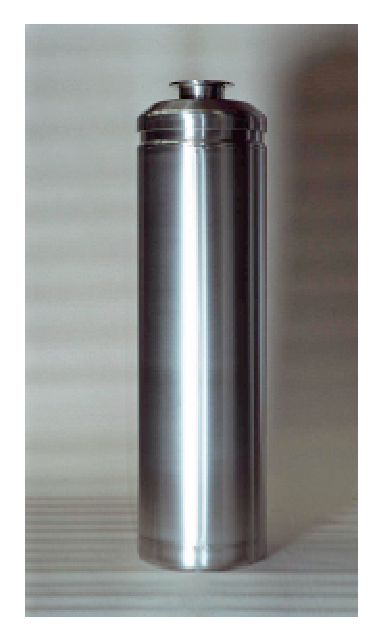
\includegraphics[width = 0.3 \textwidth]{Andra1}
\end{figure}
\end{minipage}
\newline
\invisible<1>{
\textcolor{cadmiumgreen}{\textbf{The gas emission involves the environment degradation. \\
Prediction by the numerical analysis.}}
\vspace{-0.3 cm}
\newline
\newline
\invisible<2>{
\textcolor{cadmiumgreen}{\textbf{Study by mathematical tools this model. \\
Propose robust algorithms resolution and save computational time.}}
\vspace{-0.3 cm}
\newline
\newline
\invisible<3>{
\textcolor{midnightblue}{\textbf{Strongly non linear problem, an incomplete mathematical analysis, very complicated problem...}}
\vspace{-0.8 cm}
\newline
\newline
\invisible<4>{
\begin{center}\textbf{We study 2 problems of increasing difficulty.}
\end{center}
\invisible<5>{
}}}}}
\end{frame}
%
\begin{frame}
\frametitle{Motivation}
Consider the system of PDEs with nonlinear complementarity constraints:
\begin{equation*}
\begin{split}
\partial_t \left(\varphi(\bu)\right) + \mathcal{A}(\bu)=\mathcal{F}\\
\textcolor{electricpurple}{\mathcal{K}}(\bu) \geq 0 \quad \textcolor{carmine}{\mathcal{G}}(\bu) \geq 0 \quad \textcolor{electricpurple}{\mathcal{K}}(\bu) \cdot \textcolor{carmine}{\mathcal{G}}(\bu)=0
\end{split}
\end{equation*}
This model is used in various physical phenomena: economy, fluid mechanics, elasticity, multiphase flow.
\\
\invisible<1>{
\textbf{\textcolor{blue}{Numerical resolution:}}
\invisible<2>{
\begin{itemize}
\item Discretization: Finite elements /finite volumes + backward Euler scheme in time
\begin{equation*}
\begin{split}
\frac{\varphi(\bu_h^n)-\varphi(\bu_h^{n-1})}{t^{n}-t^{n-1}} + \mathcal{A}(\bu_h^{n})=\mathcal{F}_h^{n-1}\\
\textcolor{electricpurple}{\mathcal{K}}(\bu_h^{n}) \geq 0 \quad \textcolor{carmine}{\mathcal{G}}(\bu_h^{n}) \geq 0 \quad \textcolor{electricpurple}{\mathcal{K}}(\bu_h^{n}) \cdot \textcolor{carmine}{\mathcal{G}}(\bu_h^{n})=0
\end{split}
\end{equation*}
\invisible<3>{
\item Nonlinear resolution: inexact semismooth Newton algorithm
\begin{equation*}
\mathbb{A}^{n,\kk-1} \bU_h^{n,\kk,\ii} + {\bm R}_h^{n,\kk,\ii} = {\bm F}^{n,\kk-1}
\end{equation*}
\end{itemize}  
\invisible<4>{}
}}}
\end{frame}
%
\begin{frame}
\frametitle{Motivation}
\textbf{\textcolor{blue}{A posteriori error estimate:}} 
\begin{equation*}
\tnorm{\bu-\bu_h^{n,\kk,\ii}} \leq \eta(\bu_h^{n,\kk,\ii}) \quad \mbox{where} \quad \tnorm{\cdot} \quad \mbox{is some norm}
\end{equation*}
\invisible<1>{
\textbf{\textcolor{blue}{Three components of the error:}}
\begin{itemize}
\item discretization error: numerical scheme (finite elements, finite volumes...)\\ \item linearization error: semismooth Newton method ($\kk$) \\
\item algebraic error: iterative algebraic solver ($\ii$)
\end{itemize}
\invisible<2>{
\textbf{\textcolor{red}{Questions:}}

Can we estimate each component of the error? \textcolor{cadmiumgreen}{\textbf{yes!}}
\\
\begin{itemize}
\item $\tnorm{\bu-\bu_h^{n,\kk,\ii}} \leq \eta_{\mathrm{disc}}^{n,\kk,\ii} + \eta_{\mathrm{lin}}^{n,\kk,\ii} + \eta_{\mathrm{alg}}^{n,\kk,\ii}$
\end{itemize}  
\invisible<3>{
Can we reduce the number of iterations? \textcolor{cadmiumgreen}{\textbf{yes!}}
\begin{itemize}
\item Adaptive stopping criterion: semismooth linearization: $\eta_{\mathrm{lin}}^{n,\kk,\ii} \leq \gamma_{\mathrm{lin}} \eta_{\mathrm{disc}}^{n,\kk,\ii}$
\item Adaptive stopping criterion: algebraic: $\eta_{\mathrm{alg}}^{n,\kk,\ii} \leq \gamma_{\mathrm{alg}} \left\{ \eta_{\mathrm{disc}}^{n,\kk,\ii}, \eta_{\mathrm{lin}}^{n,\kk,\ii} \right\}$
\end{itemize}
\invisible<4>{}
}}}
\end{frame}
%
\begin{frame}
\frametitle{Main contribution}
\vspace{-0.2 cm}
\textcolor{red}{\textbf{Stationary linear variational inequality}}

\begin{equation*}
\vspace{-0.2 cm}
\mbox{Find} \quad \bu \in \Kg \quad a(\bu,\bv-\bu) \geq (\bbf,\bv-\bu) \quad \forall \bv \in \Kg
\end{equation*}


\vspace{-0.4 cm}
\begin{figure}
\rotatebox{90}{
\includegraphics[width = 0.295\textwidth]{Biblio_intro.pdf}}
\end{figure}
\begin{thebibliography}{10}

 \scriptsize{
 \bibitem{Dabaghi:2018}
 {\sc J.~Dabaghi, V.~Martin, and M.~Vohral{\'{\i}}k}, {\em Adaptive inexact
  semismooth Newton methods for the contact problem between two membranes}.
 \textcolor{black}{HAL Preprint~01666845, submitted for publication, 2018}
 }

\end{thebibliography}
\end{frame}
%
%
\begin{frame}
\textcolor{red} {\textbf{Two-phase compositional flow in porous media}}
\vspace{-0.1 cm}
\begin{equation*}
\mbox{Find} \quad \Sl, \Pl, \chihl \quad \dps
\left\lbrace\begin{array}{llccc}
\dps \partial_t l_\componentw(\Sl) + \nab \cdot {\bm \Phi}_{\mathrm{w}}(\Sl,\Pl,\chihl) = Q_{\componentw},  \\
              \dps \partial_t l_\componenth(\Sl,\chihl)  + \nab \cdot {\bm \Phi}_{\mathrm{h}}(\Sl,\Pl,\chihl)=\Qh,\\
\textcolor{electricpurple}{\mathcal{K}}(\Sl) \geq 0, \;  \textcolor{carmine}{\mathcal{G}}(\Sl,\Pl,\chihl) \geq 0, \; \textcolor{electricpurple}{\mathcal{K}}(\Sl) \cdot \textcolor{carmine}{\mathcal{G}}(\Sl,\Pl,\chihl)=0  
\end{array}
\right.
\end{equation*}
\vspace{-0.3 cm}
\begin{figure}
\rotatebox{90}{\includegraphics[width = 0.31 \textwidth]{Biblio_intro3.pdf}}
\end{figure}
\vspace{-0.2 cm}
\begin{thebibliography}{10}
 \scriptsize{
 \bibitem{Dabaghi2:2018}
 {\sc I.~Ben Gharbia, J.~Dabaghi, V.~Martin, and M.~Vohral{\'{\i}}k}, {\em A posteriori error estimates and adaptive stopping criteria for a compositional two-phase flow with nonlinear complementarity constraints}.
 \textcolor{black}{HAL Preprint~01919067, In revision, 2019}}
 \end{thebibliography}
\end{frame}
\section{Stationary variational inequality}
\subsection{}
\begin{frame}
\frametitle{Model problem and settings: contact between two membranes}
\vspace{-1.7 cm}
\begin{equation*}
\mbox{Find} \ u_1, u_2, \lambda \ \mbox{such that} \quad
\dps
\left\lbrace\begin{array}{llccc}
\dps -\mu_1 \Delta u_1-\lambda = f_1 \qquad \mbox{in} \quad \Omega, \\
\dps -\mu_2 \Delta u_2+\lambda = f_2 \qquad \mbox{in} \quad \Omega,\\
\dps (\textcolor{electricpurple}{u_1-u_2})\textcolor{carmine}{\lambda}=0, \quad \textcolor{electricpurple}{u_1-u_2 \geq 0}, \quad 
\textcolor{carmine}{\lambda \geq 0} \qquad \mbox{in} \quad \Omega, \hspace{0.2 cm}\\
\dps u_1=g > 0 \qquad \mbox{on} \quad\partial \Omega,\\
\dps u_2=0 \qquad \mbox{on} \quad\partial \Omega.
\end{array}
\right.
%\label{eq:modele_initial_membrane}
\end{equation*}
\vspace{-0.8 cm}
\begin{figure}[t]
\begin{subfigure}[normal]{0.44\textwidth} 
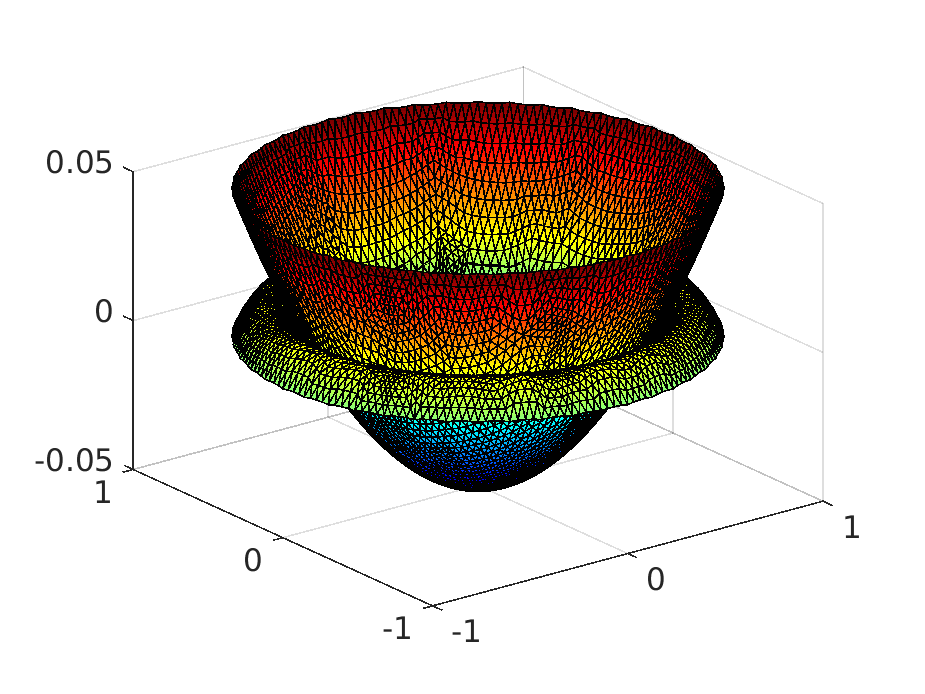
\includegraphics[width=\textwidth]{fig_article_chap_1/fig_membrane_cv.eps}    
\label{ref:position_membrane_convergence}
\end{subfigure}
\qquad
\begin{subfigure}[normal]{0.44\textwidth}
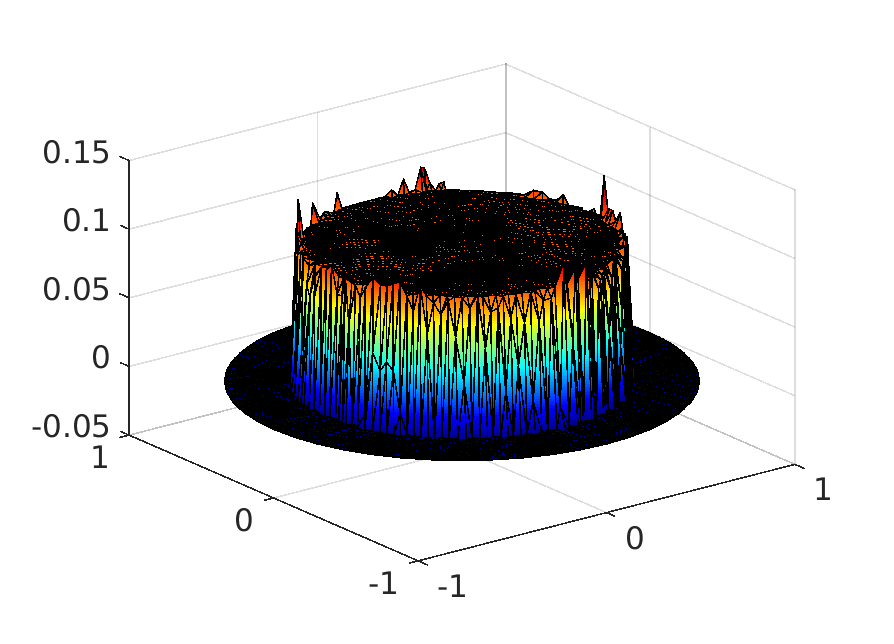
\includegraphics[width=\textwidth]{fig_article_chap_1/fig_lambda_cv.eps}     
\label{ref:lambda_membrane_convergence} 
\end{subfigure}
\end{figure}
\vspace*{-4.4cm}\hspace*{1.5 cm}$u_1$\\
\vspace*{0.7cm}\hspace*{1.5 cm}$u_2$
\end{frame}
%
\begin{frame}
\frametitle{Continuous problem}
\begin{itemize}
\item $H_g^1(\Omega)\hspace{-0.1 cm} =\hspace{-0.1 cm} \left\{u\in H^1(\Omega), \hspace{0.1 cm} u=g \hspace{0.1 cm} \mbox{on} \hspace{0.1 cm} \partial \Omega\right\}$ \quad $\Lambda=\left\{\chi\in L^2(\Omega), \: \textcolor{carmine}{\chi \geq 0} \: \mbox{on} \hspace{0.1 cm} \Omega\right\}$
\end{itemize}
\textbf{Saddle point type weak formulation:}
For $(f_1,f_2)\in \left[L^2(\Omega)\right]^2$ and $g > 0$ find $(u_1,u_2,\lambda)\in H_g^1(\Omega)\times H_0^1(\Omega) \times \Lambda$ such that
\begin{equation*}
\left\lbrace\begin{array}{llccc}
\dps \sum_{\ialf=1}^2 \mu_\ialf \left(\nab u_\ialf,\nab v_\ialf\right)_{\Omega} - \left(\lambda,v_1-v_2\right)_{\Omega} = \sum_{\ialf=1}^2\left(f_\ialf,v_\ialf\right)_{\Omega} \quad \forall (v_1,v_2) \in \left[H_0^1(\Omega)\right]^2 \\
\left(\chi - \textcolor{carmine}{\lambda},\textcolor{electricpurple}{u_1-u_2}\right)_{\Omega} \geq 0 
\quad \forall \chi \in \Lambda \hspace{7 cm} \textcolor{electricpurple}{(\mathrm{S})}
\end{array}
\right.
\end{equation*}
\hspace{4.5 cm}\textcolor{cadmiumgreen}{\textbf{equivalent to}}\\
\textbf{Variational inequality:}
\begin{itemize}
\item $\Kg= \left\{(v_1,v_2)\in H_g^1(\Omega)\times H_0^1(\Omega),\: \textcolor{electricpurple}{v_1-v_2 \geq 0} \; \; \mbox{on} 
\hspace{0.1 cm} \Omega \right\}$
\end{itemize}

\begin{equation*}
\dps \sum_{\ialf=1}^2 \mu_\ialf \left(\nab u_\ialf,\nab \left(v_\ialf-u_\ialf\right)\right)_{\Omega} \geq \sum_{\ialf=1}^2\left(f_\ialf,v_\ialf-u_\ialf\right)_{\Omega} \quad \forall \bv = (v_1,v_2)\in ~\Kg \qquad \textcolor{electricpurple}{(\mathrm{R})}
\end{equation*}
\end{frame}
%
\begin{frame}
\textcolor{red}{\textbf{For any $p \geq 1$}}
\\
\frametitle{Discretization by finite elements}
\textcolor{cadmiumgreen}{\textbf{Spaces for the discretization:}}\\
$\Xghp=\left\{v_h \in \mathcal{C}^0(\overline{\Omega}),  {v_h}_{|K} \in \Pp (K), \ \forall K \in {\mathcal{T}}_h, \hspace{0.2 cm} v_h=g \hspace{0.2 cm} \mbox{on} \hspace{0.2 cm} \partial \Omega\right\}$\\
\vspace*{0.3 cm}
$\Xzerohp =\left\{v_h \in \calC^0(\overline{\Omega}); \ {v_h}|_{K} \in \Pp (K), \quad \forall K \in \Th \right\} \cap H_0^1(\Omega)$
\\
\vspace*{0.3 cm}
$\dps \Kghp=\left\{(\vunh,\vdeuxh) \in \Xghp \times \Xzerohp, \ \textcolor{electricpurple}{\vunh(\xl)-\vdeuxh(\xl)} \geq 0 \ \ \forall \xl \in \Vdp \right\} \textcolor{red}{\not \subset \Kg \quad \forall p \geq 2}$\\
\vspace*{0.2 cm}
\invisible<1>{
\textcolor{cadmiumgreen}{\textbf{Discrete variational inequality:}} find $\dps \uh=(\uunh,\udeuxh) \in \Kghp$ such that
\begin{equation*}
\dps \sum_{\ialf=1}^2 \mu_\ialf \left(\nab u_{\ialf h},\nab \left(v_{\ialf h}-u_{\ialf h}\right)\right)_{\Omega} \geq \sum_{\ialf=1}^2\left(f_\ialf,v_{\ialf h}-u_{\ialf h}\right)_{\Omega} \quad \forall \bv_h = (v_{1h},v_{2h})\in ~\Kg \quad \textcolor{electricpurple}{(\mathrm{DR})}
\end{equation*}
\invisible<2>{
\textcolor{midnightblue}{\textbf{Resolution techniques:}}
 Projected Newton methods (Bertsekas 1982), Active set Newton method (Kanzow 1999), Primal-dual active set strategy (Hinterm\"uller 2002).\invisible<3>{
}}}
\end{frame}
%
\begin{frame}
\frametitle{Saddle point formulation}
\textcolor{cadmiumgreen}{\textbf{Characterization of the discrete lagrange multiplier:}}
Define $\lambih$ and $\lambiih$ in $\XXhp$ by
\begin{equation*}
\left\lbrace\begin{array}{rclcc}
\dps \left\langle \lambih,z_{1h}\right\rangle _h&\egaldef& \hspace{0.8em}
\dps \mu_1 \left(\nab \uunh, \nab z_{1h}\right)_{\Omega} - \left(f_1, z_{1h}\right)_{\Omega} \quad &\forall z_{1h} \in \Xzerohp,\\
\dps \left\langle \lambiih,z_{2h}\right\rangle _h&\egaldef& \dps
-\mu_2 \left(\nab \udeuxh, \nab z_{2h}\right)_{\Omega} + \left(f_2, z_{2h}\right)_{\Omega} \quad &\forall z_{2h} \in \Xzerohp,\\
\langle \lambih,\psihl \rangle_h &\egaldef &\langle \lambiih,\psihl \rangle_h =0  \quad &\forall \xl \in \Vdpext, \\
\end{array}
\right. 
\end{equation*}
where for all $\left(w_h ,v_h\right) \in \XXhp \times \XXhp$
\begin{equation*}
\left\langle w_h ,v_h \right\rangle_h \egaldef \dps \sum_{\ba \in \Vh} w_h(\ba) v_h(\ba) \Ma  \quad \mbox{if} \quad p=1 \quad \mbox{and} \quad \left \langle w_h ,v_h \right\rangle_h  \egaldef \dps \left(w_h, v_h\right)_{\Omega} \quad \mbox{if} \quad p \geq 2
\end{equation*}
\invisible<1>{
\textcolor{red}{\textbf{$p = 1$:}} \ $\Lahone \egaldef \left\{v_h \in \Xzerohone \  \textcolor{carmine}{v_h(\ba)} \geq 0 \ \forall \ba \in \Vdpint \right\} \textcolor{red}{\bm \subset \bm \Lambda}$ \scriptsize{Ben Belgacem, Bernardi, Blouza, and Vohral{\'{\i}}k (2008)}
\newline
\invisible<2>{
\normalsize{\textcolor{red}{\textbf{$p \geq 2$ (\textcolor{cadmiumgreen}{\textbf{new}}):}} \ $\Lahp \egaldef \left\{v_h \in \XXhp \ \left\langle v_h ,\psihl \right\rangle_h \geq 0 \ \forall \xl \in \Vdpint \ \left\langle v_h ,\psihl \right\rangle_h = 0 \hspace{0.05 cm} \forall \xl \in \Vdpext\right\}$ \textcolor{red}{$\bm \not \subset \bm \Lambda$} }
\invisible<3>{
}}}
\end{frame} 
%
\begin{frame}
\textcolor{cadmiumgreen}{\textbf{Discrete saddle point type formulation}}
Find $(\uunh,\udeuxh,\lambh)\in \Xghp \times \Xzerohp \times
\Lahp$ such that $\forall(z_{1h},z_{2h})\in [\Xzerohp]^2$ 
\vspace{-0.2 cm}
\begin{equation*}
\begin{array}{lcl}
\dps \sum_{\ialf=1}^2 \mu_\ialf \left(\nab u_{\ialf h}, \nab z_{\ialf h}\right)_{\Omega}
- \left\langle \lambh, z_{1h}-z_{2h} \right \rangle_h
=  \dps \sum_{\ialf=1}^2 \left(f_\ialf,z_{\ialf h}\right)_{\Omega} \quad \textcolor{electricpurple}{(\mathrm{DS})}, \\
\left\langle \chi_h - \textcolor{carmine}{\lambh}, \textcolor{electricpurple}{\uunh - \udeuxh}\right \rangle_h   \geq 0 \quad \forall \chi_h \in \Lahp.
\end{array}
\end{equation*}
\invisible<1>{
\vspace{-0.2 cm} 
\begin{lemma}
\textcolor{electricpurple}{$\mathrm{(DR)}$} \textcolor{red}{\textbf{equivalent to}} \textcolor{electricpurple}{$\mathrm{(DS)}$}
\end{lemma}
\invisible<2>{
\vspace{-0.1 cm}
\begin{itemize}
\item \textcolor{red}{\textbf{$p=1$}:}  Ben Belgacem, Bernardi, Blouza, and Vohral{\'{\i}}k (2008)
\invisible<3>{
\item \textcolor{red}{\textbf{$p \geq 2$}:} New $\rightarrow$ Construction of the basis $\left(\Thetahl\right)_{1 \leq l \leq \Ndp}$ of $\XXhp$, dual to $\left(\psihl\right)_{1 \leq l \leq \Ndp}$. 
\begin{equation*}
\left \langle \Thetahl , \psihlprime \right \rangle_h = \delta_{l}^{l^{\prime}}
\end{equation*}
\hspace{-0.9 cm} \mbox{$(\uunh,\udeuxh,\lambh)$ solution of \textcolor{electricpurple}{$\mathrm{(DS)}$} $\Rightarrow \left\langle \chi_h, \uunh-\udeuxh \right \rangle_h \geq 0 \ \forall \chi_h \in \Lahp$. Take $\chi_h = \Thetahl$, $\xl \in \Vdpint$} 
\begin{equation*}
\sum_{\xl^{\prime} \in \Vdp} \left(\uunh-\udeuxh\right)(\xl^{\prime}) \left\langle \Thetahl,  \psihlprime\right \rangle_h = \textcolor{carmine}{ \left(\uunh-\udeuxh\right)(\bx_l^{\prime}) \geq 0} \Rightarrow \uh \in \Kghp
\end{equation*}
\end{itemize}
\invisible<4>{
}}}}
\end{frame}
%
\begin{frame}
\frametitle{Discrete complementarity problems}
\vspace{-1 cm}
\begin{equation*}
\begin{array}{lcl}
\dps \sum_{\ialf=1}^2 \mu_\ialf \left(\nab u_{\ialf h}, \nab z_{\ialf h}\right)_{\Omega}
- \left\langle \lambh, z_{1h}-z_{2h} \right \rangle_h
=  \dps \sum_{\ialf=1}^2 \left(f_\ialf,z_{\ialf h}\right)_{\Omega} \quad \forall(z_{1h},z_{2h})\in [\Xzerohp]^2, \\
\textcolor{electricpurple}{\left(\uunh-\udeuxh \right)(\xl)} \geq 0 \ \forall \xl \in \Vdpint, \ \left\langle \textcolor{carmine}{\lambh}, \psihl \right \rangle_h \geq 0 \ \forall \xl \in \Vdpint, \ \left\langle \textcolor{carmine}{\lambh}, \textcolor{electricpurple}{\uunh - \udeuxh} \right \rangle_h=0.
\end{array}
\end{equation*} 
\textcolor{cadmiumgreen}{\textbf{Expression of the discrete problem in the Lagrange basis and in the dual basis:} }
\newline
\newline
\begin{onlyenv}<1>
\textcolor{red}{\textbf{$p=1$: Lagrange basis:}} $\uunh = \uunhzero + g$ where $\uunhzero \in \Xzerohp$ and $g > 0$. 
\beeqn
\uunh = \sum_{l=1}^{\Nhint} \left(\X_{1h} \right)_l \psihl + g, \quad \udeuxh = \sum_{l=1}^{\Nhint} \left(\X_{2h} \right)_l \psihl \in \Xzerohp \quad \lambh = \sum_{l=1}^{\Nhint} \left(\X_{3h} \right)_l \psihal \in \Xzerohp, 
\eeqn
\begin{equation*}
\begin{split}
&\bbE _1 \Xh = \bF,\\
&\textcolor{electricpurple}{\X_{1h} + g {\bf 1} - \X_{2h}} \geq 0, \quad \textcolor{carmine}{\X_{3h}} \geq 0, \quad \left(\textcolor{electricpurple}{\X_{1h} + g {\bf 1} - \X_{2h}} \right) \cdot \textcolor{carmine}{\X_{3h}} = 0.
\end{split}
\quad 
\bbE _1
\egaldef
\left[\begin{array}{ccr}
\mu_1 \bbS & \mathbf{0} & -\mathbb{D} \\
\mathbf{0} &\mu_2 \bbS & + \mathbb{D}
\end{array}
\right]
\end{equation*}
\end{onlyenv}
\begin{onlyenv}<2>
 \textcolor{red}{\textbf{$p \geq 2$: Lagrange basis:}}
The discrete lagrange multiplier $\lambh$ is decomposed in the full space $\XXhp$ as 
\beeqn
\lambh = \sum_{l=1}^{\Ndp} \left(\widetilde{\X}_{3h}\right)_l \psihl \quad \mbox{with} \quad \widetilde{\X}_{3h} \in \R^{\Ndp}.
\eeqn
\beeqn
\begin{split}
&\widetilde{\bbE}_p \Xh = \bF,\\
&\textcolor{electricpurple}{\X_{1h} + g {\bf 1} - \X_{2h}} \geq 0
, \quad \textcolor{carmine}{\widehat{\mathbb{M}} \widetilde{\X}_{3h}} \geq 0, \quad 
\left(\textcolor{electricpurple}{\X_{1h} + g {\bf 1} - \X_{2h}} \right) \cdot \textcolor{carmine}{\widehat{\mathbb{M}} \widetilde{\X}_{3h}} = 0.
\end{split}
\widetilde{\bbE}_p
\egaldef
\left[\begin{array}{ccr}
\mu_1 \bbS & \mathbf{0} & -\widehat{\mathbb{M}} \\
\mathbf{0} &\mu_2 \bbS & + \widehat{\mathbb{M}}
\end{array}
\right]
\eeqn
\end{onlyenv}
\begin{onlyenv}<3>
\textcolor{red}{\textbf{$p \geq 2$: Dual basis:}}
The discrete Lagrange multiplier $\lambh$ is decomposed in the basis $\Thetahl$ as
\beeqn
\lambh = \sum_{l=1}^{\Ndpint} \left(\X_{3h} \right)_l \Thetahl, \quad \mbox{with} \quad \X_{3h} \in \R^{\Ndpint}.
\eeqn
\beeqn
\begin{split}
& \bbE_{p} \Xh = \bF,\\
& \textcolor{electricpurple}{\X_{1h} + g {\bf 1} - \X_{2h}} \geq 0, \quad \textcolor{carmine}{\X_{3h}} \geq 0, \quad \left(\textcolor{electricpurple}{\X_{1h} + g {\bf 1} - \X_{2h}}\right) \cdot \textcolor{carmine}{\X_{3h}}=0. 
\end{split}
\qquad 
\bbE_{p}
\egaldef
\left[\begin{array}{ccr}
\mu_1 \bbS & \mathbf{0} & - \mathbb{I}_{\mathrm{d}}\\
\mathbf{0} &\mu_2 \bbS & + \mathbb{I}_{\mathrm{d}}
\end{array}
\right]
\eeqn
\end{onlyenv}
\end{frame}
%
\begin{frame}
 \begin{center}
 \Huge{\textcolor{carmine}{Resolution}}
\end{center}

\end{frame}
%\begin{frame}
%\begin{onlyenv}<1>
%slide1
% \end{onlyenv}
% \begin{onlyenv}<2>
% slide2
% \end{onlyenv}
% \begin{onlyenv}<3>
% slide3
% \end{onlyenv}
% \begin{onlyenv}<4>
% slide4
% \end{onlyenv}
% \end{frame}
%
%
\begin{frame}
\frametitle{C-functions}
\begin{definition}
$f: \left(\R^m\right)^2  \rightarrow \R^m$ ($m \geq 1$) is a
$C$-function or a complementarity function if
\begin{equation*}
\forall(\bx,\by)\in \left(\R^m\right)^2
\qquad f(\bx,\by)=\mathbf{0} \quad \iff \quad
\bx \geq \mathbf{0}, \quad \by \geq \mathbf{0}, \quad \bx {\cdot} \by=0.
\end{equation*}
\end{definition}
Examples of $C$-functions are the $\min$ function
\begin{equation*}
\left(\min \{\bx, \by\}\right)_l \egaldef \min \left\{\bx_l, \by_l\right\} \qquad l = 1,\dots, m,
\end{equation*}
the Fischer--Burmeister function
\begin{equation*}
\left(f_{\mathrm{FB}}(\bx,\by)\right)_l \egaldef \sqrt{\bx_l^2+\by_l^2}-\left(\bx_l+\by_l\right) \quad  l = 1,\dots, m,
\end{equation*}
or the Mangasarian function
\begin{equation*}
\left(f_{\mathrm{M}}(\bx,\by)\right)_l \egaldef \xi (|\bx_l-\by_l|) - \xi(\by_l) - \xi(\bx_l)  \quad  l = 1,\dots, m, 
\end{equation*}
where $\xi: \R \mapsto \R$ is an increasing function satisfying $\xi(\bm 0)=\bm 0$. 
\end{frame}
%
\begin{frame}
Let
$\tilde \CFun$ be any $C$-function, \ie, satisfying (for $m=\Ndpint$)
\begin{equation*}
\tilde \CFun(\textcolor{electricpurple}{\X_{1h} + g {\bf 1} - \X_{2h}}, \textcolor{carmine}{\X_{3h}})= 0 \iff \textcolor{electricpurple}{\X_{1h} + g {\bf 1} - \X_{2h}} \geq 0, \textcolor{carmine}{\X_{3h}} \geq 0, \  \left(\textcolor{electricpurple}{\X_{1h} + g {\bf 1} - \X_{2h}}\right) \cdot \textcolor{carmine}{X_{3h}} = 0.
\end{equation*} 
Then, introducing the function $\CFun:\R^{3 \Ndpint} \rightarrow \R^{\Ndpint}$ defined as
\begin{equation*}
\CFun(\X_{h})
= \tilde \CFun(\textcolor{electricpurple}{\X_{1h} + g {\bf 1} - \X_{2h},} \textcolor{carmine}{\X_{3h}})
\end{equation*}
Our problem
can be equivalently rewritten as
\begin{equation*}
\left\lbrace\begin{array}{llccc}
\bbE_{p} \X_{h} &= \bF,\\
\CFun(\X_{h})&=\mathbf{0}.
\end{array}
\right.
\end{equation*}
\textcolor{red}{\textbf{The C-function is not Fréchet differentiable.}}\\
\vspace{0.2 cm}
\textcolor{red}{\textbf{How can we solve the nonlinear problem?}}
\end{frame}
%
\begin{frame}
\frametitle{Inexact semismooth Newton method}
\begin{onlyenv}<1>
\textcolor{cadmiumgreen}{\textbf{Newton initial vector:}} $\Xh^{\zzero} \egaldef \left(\X_{1h}^{\zzero},\X_{2h}^{\zzero}, \X_{3h}^{\zzero} \right)^{T} \in \R^{3 \Ndpint}$, on step $\kk \geq 1$, one looks for $\Xh^{\kk} \in \R^{3 \Ndpint}$ such that
\begin{equation*}
\bbA^{\kk-1}\Xh^{\kk}=\bB^{\kk-1},
\end{equation*} 
where 
%the square matrix $\bbA^{\kk-1}$ and the right-hand side vector $\bB^{\kk-1}$ are respectively defined by
\begin{equation*}
\dps \bbA^{\kk-1}\egaldef
\left[\begin{array}{c}
\bbE_{p} \\
\JacCFun(\Xh^{\kk-1})
\end{array}
\right],
\quad  \hspace{0.1 cm} \bB^{\kk-1} \egaldef
\left[\begin{array}{c}
\bF\\
\JacCFun(\Xh^{\kk-1})\Xh^{\kk-1}-\CFun(\Xh^{\kk-1})
\end{array}
\right].
%\quad  \forall k\geq 1.
\end{equation*}
\end{onlyenv}
\begin{onlyenv}<2>
\textcolor{cadmiumgreen}{\textbf{Newton initial vector:}} $\Xh^{\zzero} \egaldef \left(\X_{1h}^{\zzero},\X_{2h}^{\zzero}, \X_{3h}^{\zzero} \right)^{T} \in \R^{3 \Ndpint}$, on step $\kk \geq 1$, one looks for $\Xh^{\kk} \in \R^{3 \Ndpint}$ such that
\begin{equation*}
\bbA^{\kk-1}\Xh^{\kk}=\bB^{\kk-1},
\end{equation*} 
where 
%the square matrix $\bbA^{\kk-1}$ and the right-hand side vector $\bB^{\kk-1}$ are respectively defined by
\begin{equation*}
\dps \bbA^{\kk-1}\egaldef
\left[\begin{array}{c}
\bbE_{p} \\
\JacCFun(\Xh^{\kk-1})
\end{array}
\right],
\quad  \hspace{0.1 cm} \bB^{\kk-1} \egaldef
\left[\begin{array}{c}
\bF\\
\JacCFun(\Xh^{\kk-1})\Xh^{\kk-1}-\CFun(\Xh^{\kk-1})
\end{array}
\right].
%\quad  \forall k\geq 1.
\end{equation*}
\textcolor{cadmiumgreen}{\textbf{Inexact solver initial vector:}}
$\Xh^{\kk,\izzero} \in \R^{3 \Ndpint}$, often taken as $\Xh^{\kk,\izzero} = \Xh^{\kk-1}$, this yields on step $\ii \geq
1$ an approximation $\Xh^{\kk,\ii}$ to $\Xh^{\kk}$ satisfying
\begin{equation*}
\bbA^{\kk-1}\Xh^{\kk,\ii} =\bB^{\kk-1}-{\bm R}_h^{\kk,\ii},
\end{equation*}
where ${\bm R}_h^{\kk,\ii} \in \R^{3 \Ndpint}$ is the algebraic residual vector.
\end{onlyenv}

\begin{onlyenv}<3>
\begin{center}
\Huge{\textcolor{carmine}{A posteriori error estimates}}
\end{center}
\end{onlyenv}
\end{frame}
%
\begin{frame}
\frametitle{A posteriori analysis}
\begin{equation*}
\tnorm{\bu-\bu_h^{\kk,\ii}}_{\Omega} \egaldef \left(\sum_{\ialf = 1}^2 \mu_\ialf \left\|\nab \left(\uialf-\uialfh^{\kk,\ii} \right)\right\|_{\Omega}^2 \right)^{\frac{1}{2}} \leq \eta^{\kk,\ii} \egaldef \left(\sum_{K \in Th}\left[\eta_{K}(\bu_h^{\kk,\ii})^{2} \right]^2\right)^{\frac{1}{2}}
\end{equation*}
\begin{itemize}
\item $\eta_{K}(\bu_h^{\kk,\ii})$ local estimator depending on the approximate solution 
\item $\eta^{\kk,\ii} \leq \eta_{\mathrm{disc}}^{\kk,\ii} + \eta_{\mathrm{lin}}^{\kk,\ii} + \eta_{\mathrm{alg}}^{\kk,\ii}$: identification of the error components
\item $\eta_{K}(\bu_h^{\kk,\ii}) \leq \tnorm{\bu-\bu_h^{\kk,\ii}}_{\zeta_K}$: local efficiency
\item adaptive inexact stopping criteria based on the error components
\end{itemize} 
\invisible<1>{
\textcolor{red}{We employ the methodology of equilibrated flux reconstruction to obtain local error estimators.}
\newline 
\footnotesize{Destuynder \& M\'etivet (1999) Braess \& Sch\"oberl (2008), Ern \& Vohral{\'{\i}}k (2013)}
\invisible<2>{
}}
\end{frame}
%
\begin{frame}
\frametitle{Component flux reconstruction}
\textcolor{cadmiumgreen}{\textbf{Motivation:}}
\begin{equation*}
-\mu_\ialf \nab u_{\ialf} \in \HdivOmeg,  \quad  -\mu_\ialf \nab u_{\ialf h}^{\kk,\ii} \not \in \HdivOmeg, \quad \nab \cdot \left(-\mu_\ialf \nab u_{\ialf h}^{\kk,\ii} \right) \neq f_\ialf -(-1)^{\ialf} \lambh^{\kk,\ii}
\end{equation*}
\invisible<1>{
\textcolor{cadmiumgreen}{\textbf{Flux reconstruction:}}
\begin{equation*}
{\bm \sigma}_{\ialf h}^{\kk,\ii} \in \HdivOmeg \quad \left(\nab \cdot {\bm \sigma}_{\ialf h}^{\kk,\ii}, 1 \right)_K = \left( f_\ialf -(-1)^{\ialf} \lambh^{\kk,\ii}, 1  \right)_K 
\end{equation*}
\invisible<2>{
\textcolor{cadmiumgreen}{\textbf{Decomposition of the flux:}}
\begin{equation*}
{\bm \sigma}_{\ialf h}^{\kk,\ii}  = {\bm \sigma}_{\ialf h, \mathrm{alg}}^{\kk,\ii} + {\bm \sigma}_{\ialf h, \mathrm{disc}}^{\kk,\ii}
\end{equation*}
\invisible<3>{
\textcolor{cadmiumgreen}{\textbf{Algebraic flux reconstruction:}}
\begin{equation*}
{\bm \sigma}_{\ialf h, \mathrm{alg}}^{\kk,\ii} \in \HdivOmeg \quad \nab {\cdot} {\bm \sigma}_{\ialf h, \mathrm{alg}}^{\kk,\ii}=r_{\ialf h}^{\kk,\ii} \quad \mbox{where} \quad r_{\ialf h}^{\kk,\ii} \quad \mbox{is the functional representation of} \quad {\bm R}_{\ialf h}^{\kk,\ii}
\end{equation*}
\footnotesize{Pape{\v z}, R{\"u}de, Vohral{\'{\i}}k and Wohlmuth. Submitted for publication (2017).}
\newline
\newline
\invisible<4>{
\textcolor{cadmiumgreen}{\textbf{Discretization flux reconstruction:}}
\begin{equation*}
{\bm \sigma}_{\ialf h, \mathrm{disc}}^{\kk,\ii} \in \HdivOmeg \quad \left(\nab \cdot {\bm \sigma}_{\ialf h,\mathrm{disc}}^{\kk,\ii}, 1 \right)_K = \left( f_\ialf -(-1)^{\ialf} \lambh^{\kk,\ii} - r_{\ialf h}^{\kk,\ii}, 1  \right)_K
\end{equation*}
\invisible<5>{
}}}}}
\end{frame}
%
%%%%ALG FLUX RECONSTRUCTION
% \begin{frame}
% \frametitle{Algebraic flux reconstruction}
% \vspace*{-0.5 cm}
% \begin{equation*}
% \begin{array}{lclcc}
% \left({\bm \sigma}_{\ialf j,\mathrm{alg}}^{\kk,\ii,\ba}, \tauj\right)_{\omajminusun}-\left(\gamma_{\ialf j}^{\kk,\ii,\ba},\nab {\cdot} \tauj\right)_{\omajminusun} &=& 0 & \forall \tauj\in \Vspacejjmuna, \\
% \left(\nab {\cdot} {\bm \sigma}_{\ialf j,\mathrm{alg}}^{\kk,\ii,\ba}, q_{j}\right)_{\omajminusun}&=&\dps\left(\tilde{g}_{\ialf j}^{\kk,\ii,\ba}, q_{j}\right)_{\omajminusun} & \forall q_{j} \in \Qspacejjmuna,
% \end{array}
% \end{equation*}
% \vspace{-0.8 cm}
% \begin{minipage}[c]{.55 \linewidth}
% \vspace{-0.8 cm}
% \begin{equation*}
% \begin{split}
% \Vspacejjmuna &\egaldef \left\{ \tauj \in \RTp(\omajminusun),
% \ \tauj {\cdot} \nnomajminusun =0 \mbox{ on } \partial \omajminusun \right\}, \\
% \Qspacejjmuna &\egaldef \Pp^{0}({\omajminusun}), \ \ba \in \mathcal{V}_{j-1}^{\mathrm{int}}
% \end{split}
% \end{equation*}
% \vspace{-0.2 cm}
% \invisible<1-2>{
% \begin{equation*}
% \begin{split}
% \Vspacejjmuna & \egaldef\left\{ \tauj \in \RTp(\omajminusun),
% \ \tauj {\cdot} \nnomajminusun=0 \  \mbox{on} \ \partial \omajminusun \backslash \partial \Omega\right\},
% \\
% \Qspacejjmuna & \egaldef \Pp({\omajminusun}), \ \ba \in \mathcal{V}_{j-1}^{\mathrm{ext}}
% \end{split}
% \end{equation*}
% }
% \end{minipage}
% \hfill
% \begin{minipage}[c]{.42 \linewidth}
% \hspace{3 cm}
% \begin{figure}
%   \begin{overprint}
%     \onslide<1>\includegraphics[width=0.9 \textwidth]{patch_alg_1.pdf}
%     \onslide<2>\includegraphics[width=0.9 \textwidth]{patch_alg_2.pdf}
%     \onslide<3>\includegraphics[width=0.9 \textwidth]{patch_alg_2_bis.pdf}
%     \onslide<4>\includegraphics[width=0.9 \textwidth]{patch_alg_3.pdf}
%     \onslide<5->\includegraphics[width=0.9 \textwidth]{patch_alg_4.pdf} 
%     \end{overprint}
% \end{figure}
% \end{minipage}
% \vspace{-0.2 cm}
% \invisible<1-4>{
% \begin{equation*}
% {\bm \sigma}_{\ialf j,\mathrm{alg}}^{\kk,\ii} \egaldef \sum_{j=1}^{J} \sum_{\ba \in \mathcal{V}_{j-1}} {\bm \sigma}_{\ialf j,\mathrm{alg}}^{\kk,\ii,\ba}
% \end{equation*}
% }
% \end{frame}
%
\begin{frame}
\frametitle{Discretization flux reconstruction}
\vspace{-0.4 cm}
\begin{equation*}
\begin{array}{lclcc}
\left({\bm \sigma}_{\ialf h, \mathrm{disc}}^{\kk,\ii,\ba}, \tauh\right)_{\omah}- \left(\gamma_{\ialf h}^{\kk,\ii,\ba},\nab {\cdot} \tauh\right)_{\omah}
&=& -\left(\mu_\ialf \psiha \nab u_{\ialf h}^{\kk,\ii,\ba}, \tauh \right)_{\omega_h^{\ba}}
&  \forall \tauh\in \Vspaceha, \\
\left(\nab {\cdot} {\bm \sigma}_{\ialf h, \mathrm{disc}}^{\kk,\ii, \ba}, q_{h}\right)_{\omah}
&=&\left(\tilde{g}_{\ialf h}^{\kk,\ii,\ba}, q_{h}\right)_{\omah}
&  \forall q_{h}\in \Qspaceha,
\end{array}
\end{equation*}

\begin{minipage}[c]{0.4 \linewidth}
$ \ba \in \Vhint$
\vspace{-0.2 cm}
\begin{equation*}
\begin{split}
\Vspaceha & \egaldef
 \left\{\tauh  \in \RTp(\omah), \, \tauh {\cdot} \nnomah=0  \mbox{ on } \partial \omah \right\}\\
\Qspaceha &  \egaldef \Pp^{0}(\omah)
\end{split}
\vspace{-0.2 cm}
\end{equation*}
\invisible<1>{
\begin{equation*}
{\bm \sigma}_{\ialf h, \mathrm{disc}}^{\kk,\ii} \egaldef \sum_{\ba \in \mathcal{V}_h} {\bm \sigma}_{\ialf h, \mathrm{disc}}^{\kk,\ii,\ba}
\end{equation*}
}
\end{minipage}
\hfill
\begin{minipage}[c]{0.5 \linewidth}
\begin{figure}
  \begin{overprint}
    \onslide<1>\includegraphics[width=0.9\textwidth]{patch_alg_3.pdf}
    \onslide<2->\includegraphics[width=0.9\textwidth]{patch_alg_5.pdf}
    \end{overprint}
\end{figure}
\end{minipage}
\end{frame}
%
\begin{frame}
\frametitle{Estimators}

\textcolor{cadmiumgreen}{\textbf{Violations of physical properties of the numerical solution}}
\begin{equation*}
{\bm \sigma}_{\ialf h}^{\kk,\ii} \neq -\nab \uialfh^{\kk,\ii} \quad \nab \cdot \left(-\mu_\ialf \nab u_{\ialf h}^{\kk,\ii} \right) \neq f_\ialf -(-1)^{\ialf} \lambh^{\kk,\ii}
\end{equation*}
\invisible<1>{
\textcolor{midnightblue}{\textbf{Flux estimator:}}
\begin{equation*}
\eta_{\mathrm{F},K,\ialf}^{\kk,\ii} \egaldef \left\|\mu_\ialf^{\frac{1}{2}} \nab u_{\ialf h}^{\kk,\ii}
+\mu_\ialf^{-\frac{1}{2}} {\bm \sigma}_{\ialf h}^{\kk,\ii}\right\|_{K},
\end{equation*}
\textcolor{midnightblue}{\textbf{Residual estimator:}}
\begin{equation*}
\eta_{\mathrm{R},K,\ialf}^{\kk,\ii} \egaldef \frac{h_K}{\pi} \mu_\ialf^{-\frac{1}{2}}
\left\|f_\ialf - \nab \cdot {\bm \sigma}_{\ialf h}^{\kk,\ii} -(-1)^{\ialf} \lambh^{\kk,\ii} \right\|_{K},
\end{equation*}
\invisible<2>{
\textcolor{cadmiumgreen}{ \textbf{Violations of the complementarity constraints}} 
\begin{equation*}
\textcolor{red}{p = 1:} (\uunh^{\kk,\ii}-\udeuxh^{\kk,\ii})(\ba) \not \geq 0 \quad \lambh^{\kk,\ii}(\ba) \not \geq 0 \quad \lambh^{\kk,\ii}(\ba) \cdot (\uunh^{\kk,\ii}-\udeuxh^{\kk,\ii})(\ba)\not=0 \quad \forall \ba \in \Vhint
\end{equation*}
\begin{equation*}
\textcolor{red}{p \geq 2:}
(\uunh^{\kk,\ii} - \udeuxh^{\kk,\ii})(\bx_l) \not \geq 0 \ , \ \left(\lambh^{\kk,\ii},\psihl \right)_{\Omega} \not \geq 0 \ \forall \bx_l \in \Vdpint \ \left(\lambh^{\kk,\ii},\uunh^{\kk,\ii}-\udeuxh^{\kk,\ii}\right)_{\Omega} \neq 0
\end{equation*}
\invisible<3>{
}}}
\end{frame}
%
\begin{frame}
\textcolor{red}{\textbf{Strategy for constructing the estimators}}
\begin{equation*}
%\label{eq:def:lambda:pos:neg}
\lambh^{\kk,\ii} \egaldef \lambh^{\kk,\ii,\mathrm{pos}} + \lambh^{\kk,\ii,\mathrm{neg}}, \quad \Ktildeghp \egaldef \left\{(\vunh,\vdeuxh) \in \Xghp \times \Xzerohp, \ \textcolor{electricpurple}{\vunh-\vdeuxh} \geq 0  \right\} \subset \Kg.
\end{equation*}
\invisible<1>{
\textcolor{midnightblue}{\textbf{Contact estimator:}}
\begin{equation*}
\eta_{\mathrm{C},K}^{\kk,\ii,\mathrm{pos}} \egaldef 2 \left(\lambh^{\kk,\ii,\mathrm{pos}},\uunh^{\kk,\ii}-\udeuxh^{\kk,\ii} \right)_K,
\end{equation*}
\invisible<2>{
\textcolor{midnightblue}{\textbf{Nonconformity estimator 1:}}
\begin{equation*}
\eta_{\mathrm{nonc},1,K}^{\kk,\ii}  \egaldef  \tnorm{{\bm s}_h^{\kk,\ii}-\uh^{\kk,\ii}}_K, 
\end{equation*}
\vspace{-0.1 cm}
\invisible<3>{
\textcolor{midnightblue}{\textbf{Nonconformity estimator 2:}}
\begin{equation*}
\eta_{\mathrm{nonc},2,K}^{\kk,\ii} \egaldef h_{\Omega} \CPF \left(\frac{1}{\mu_1} +
\frac{1}{\mu_2} \right)^{\frac{1}{2}} \left\| \lambh^{\kk,\ii,\mathrm{neg}}\right\|_K, 
\end{equation*}
\invisible<4>{
\vspace{-0.2 cm}
\textcolor{midnightblue}{\textbf{Nonconformity estimator 3:}}
\begin{equation*}
\eta_{\mathrm{nonc},3,K}^{\kk,\ii}  \egaldef 2 h_{\Omega} \CPF \left(\frac{1}{\mu_1} +
\frac{1}{\mu_2} \right)^{\frac{1}{2}} \left\|\lambh^{\kk,\ii,\mathrm{pos}}\right\|_{\Omega}
\tnorm{{\bm s}_{h}^{\kk,\ii}-\uh^{\kk,\ii}}_K.
\end{equation*}
\invisible<5>{
}}}}}
\end{frame}
%
\begin{frame}
\begin{theorem}[A posteriori error estimate]
\begin{equation*}
\tnorm{\bu-\uh^{\kk,\ii}} \leq \hspace{-0.1 cm}
\left\{ \left(\left(\sum_{K \in \Th} \sum_{\ialf = 1}^2
\left(\eta_{\mathrm{F},K,\ialf}^{\kk,\ii} \hspace{-0.1 cm}+\hspace{-0.05 cm} \eta_{\mathrm{R},K,\ialf}^{\kk,\ii} \right)^2 \right)^{\frac{1}{2}} \hspace{-0.1 cm}+ \hspace{-0.05 cm}\eta_{\mathrm{nonc},1}^{\kk,\ii} + \eta_{\mathrm{nonc},2}^{\kk,\ii} \right)^2
\hspace{-0.1 cm}+ \hspace{-0.05 cm} \eta_{\mathrm{nonc},3}^{\kk,\ii} + \hspace{-0.1 cm}\sum_{K\in\Th} \hspace{-0.1 cm} \eta_{\mathrm{C},K}^{\kk,\ii,\mathrm{pos}} \right\}^{\frac{1}{2}}
\end{equation*}
\end{theorem}
\vspace{-0.1 cm}
\invisible<1>{
\begin{corollary}[Distinction of the error components]
\begin{equation*}
\tnorm{\bu-\uh^{\kk,\ii}} \leq \eta_{\mathrm{disc}}^{\kk,\ii} + \eta_{\mathrm{lin}}^{\kk,\ii} + \eta_{\mathrm{alg}}^{\kk,\ii}
\end{equation*}
\end{corollary}
\invisible<2>{
\begin{minipage}[c]{.32 \textwidth}
\textcolor{red}{\textbf{Adaptive algorithm}}
\\
 \textbf{If} \fcolorbox{violet}{white}{$\eta_{\mathrm{alg}}^{\kk,\ii} \leq \gamma_{\mathrm{alg}} \max  \left\{{\eta_{\mathrm{disc}}^{\kk,\ii}, \eta_{\mathrm{lin}}^{\kk,\ii}}\right\}$} \\
 \qquad  \textbf{Stop linear solver}	
\\
  \textbf{If} \fcolorbox{violet}{white}{ $\eta_{\mathrm{lin}}^{\kk,\ii} \leq \gamma_{\mathrm{lin}} \eta_{\mathrm{disc}}^{n,\kk,\ii}$}
\\
 \qquad {\textbf{Stop nonlinear solver}}
\end{minipage}
\hfill
\invisible<3>{
\begin{minipage}[c]{0.65 \textwidth}
\textcolor{red}{\hspace{4 cm}\textbf{Local efficiency (shown only for p=1):}}
\begin{equation*}
\eta_{\mathrm{disc},K}^{\kk,\ii}  \lesssim \hspace{-0.1 cm}  \hspace{-0.1 cm} \sum_{\ba \in \Vh} \left(\left\|\mu_{\ialf}^{\frac{1}{2}} \nab \left(\uialf \hspace{-0.1 cm} - \hspace{-0.1 cm} \uialfh^{\kk,\ii} \right)  \right\|_{\omah} \hspace{-0.15 cm} + \hspace{-0.1 cm} \tnorm{\lambda \hspace{-0.1 cm} - \hspace{-0.1 cm} \lambda_h^{\kk,\ii}(\ba)}_{H^{-1}_{*}(\omah)}\right)
\end{equation*}
\end{minipage}
 \invisible<4>{
}}}}
\end{frame}
%
\begin{frame}
\centering
\Huge{\textcolor{carmine}{Numerical experiments}}
\end{frame}
%
\begin{frame}
\frametitle{Numerical experiments}

\begin{itemize}
\item
$\Omega$ = \mbox{unit disk}, $J = 3$, $\mu_1= \mu_2 = 1$, $g = 0.05$, $\gamma_{\mathrm{lin}}=0.3$ $\gamma_{\mathrm{alg}}=0.3$
\item 
semismooth solver: \textcolor{blue}{Newton-min}. Linear solver: \textcolor{red}{GMRES} with ILU preconditionner.
\end{itemize}


\begin{figure}
\begin{minipage}[c]{.34\linewidth}
   \centering
   \quad Exact Newton
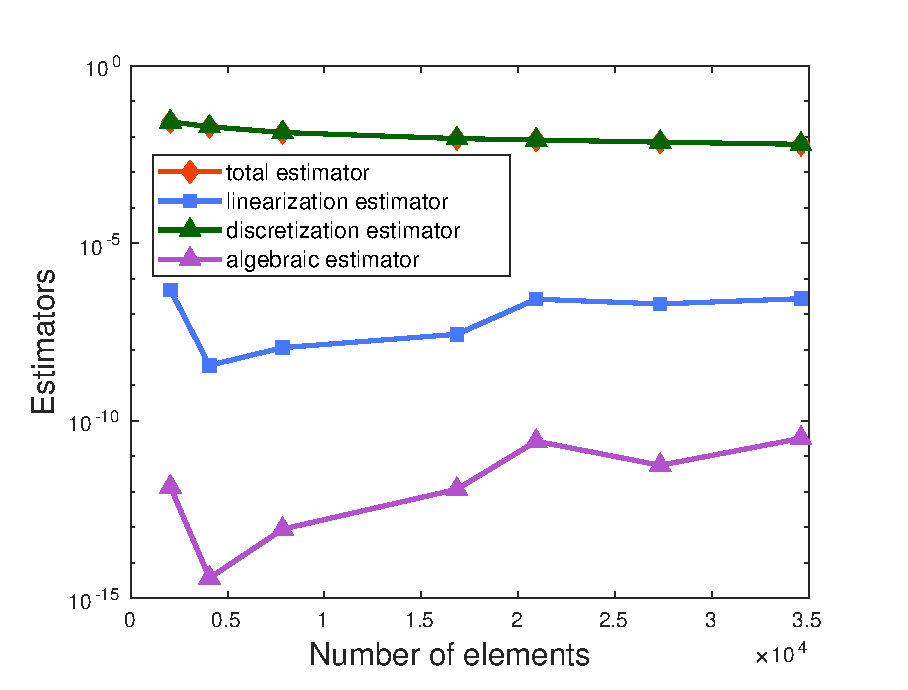
\includegraphics[width=\textwidth]{fig_article_chap_1/exact_resolution_convergence_estimator_number_elements.eps}    
%\label{ref:position_membrane_convergence}
\end{minipage}\hfill
\begin{minipage}[c]{.33\linewidth}
   \centering
   \quad Inexact Newton
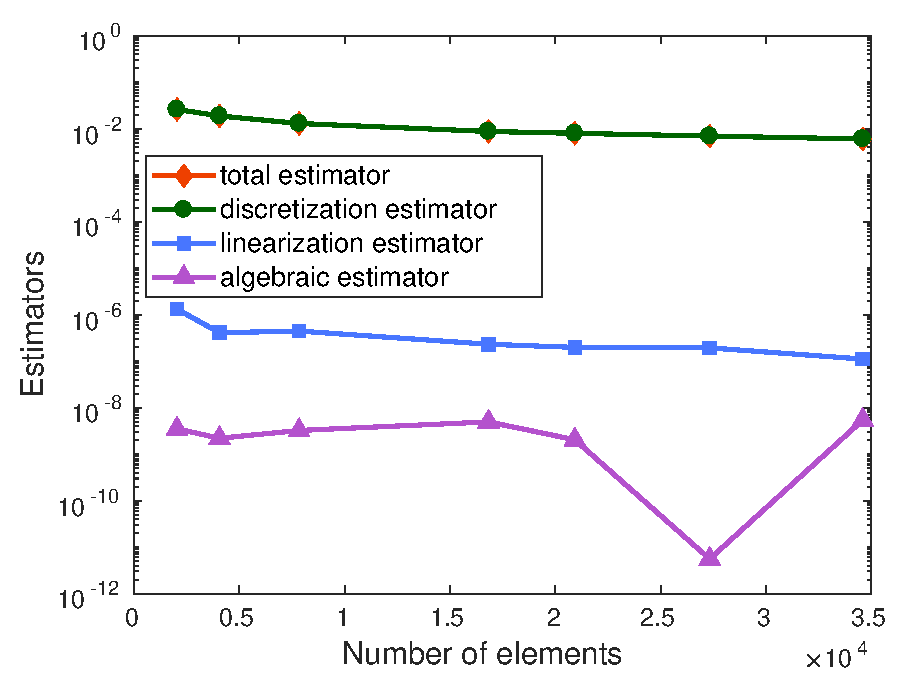
\includegraphics[width=\textwidth]{fig_article_chap_1/inexact_resolution_convergence_estimator_number_elements.eps}    
%\label{ref:position_membrane_convergence}
\end{minipage}\hfill
\begin{minipage}[c]{.33\linewidth}
   \centering
   Adaptive inexact Newton
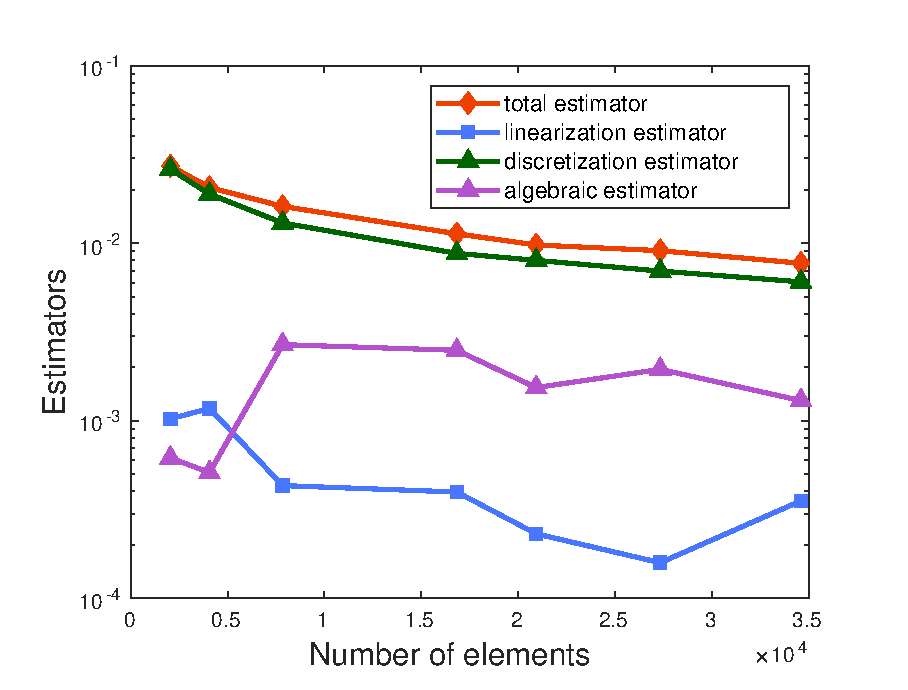
\includegraphics[width=\textwidth]{fig_article_chap_1/adapt_inexact_resolution_convergence_estimator_number_elements.eps}     
%\label{ref:lambda_membrane_convergence} 
\end{minipage}
%\caption{Exact Newton(left), Inexact Newton(middle), adaptive inexact Newton(right)}
\end{figure}

\textcolor{red}{\textbf{Quality and precision are preserved for adaptive inexact semismooth Newton method.}}


\end{frame}

\begin{frame}
\frametitle{GMRES adaptivity}
\hspace{5.5 cm} Exact/Adapt inexact Newton \hspace{3.5 cm } 
%Inexact Newton
\begin{figure}
   \centering
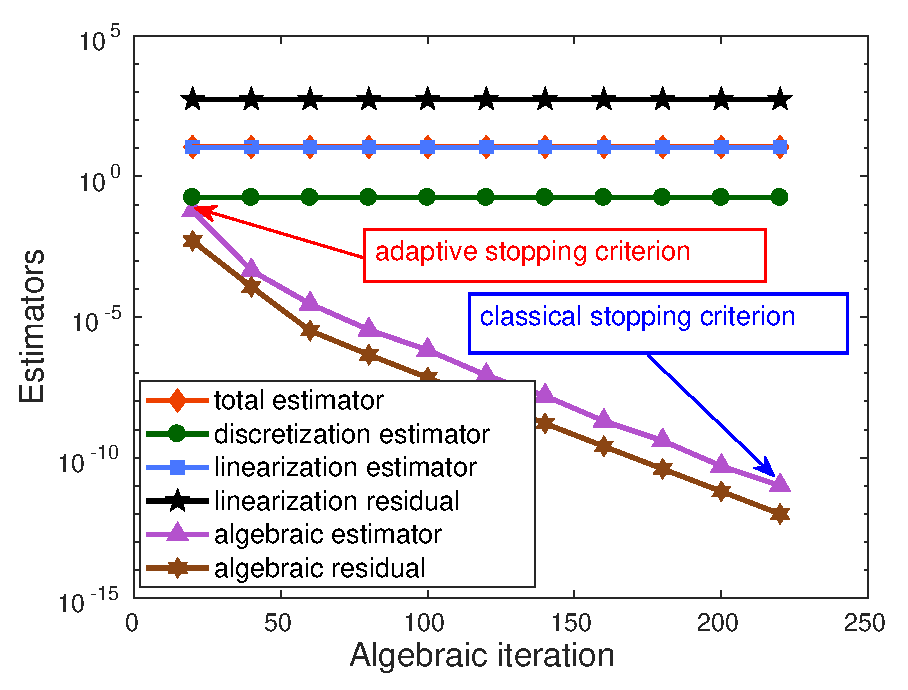
\includegraphics[width=0.50\textwidth]{fig_article_chap_1/exact_adapt_res_estimators_gmres_iter_first_newton_iter_Hmax_015.eps}    
% 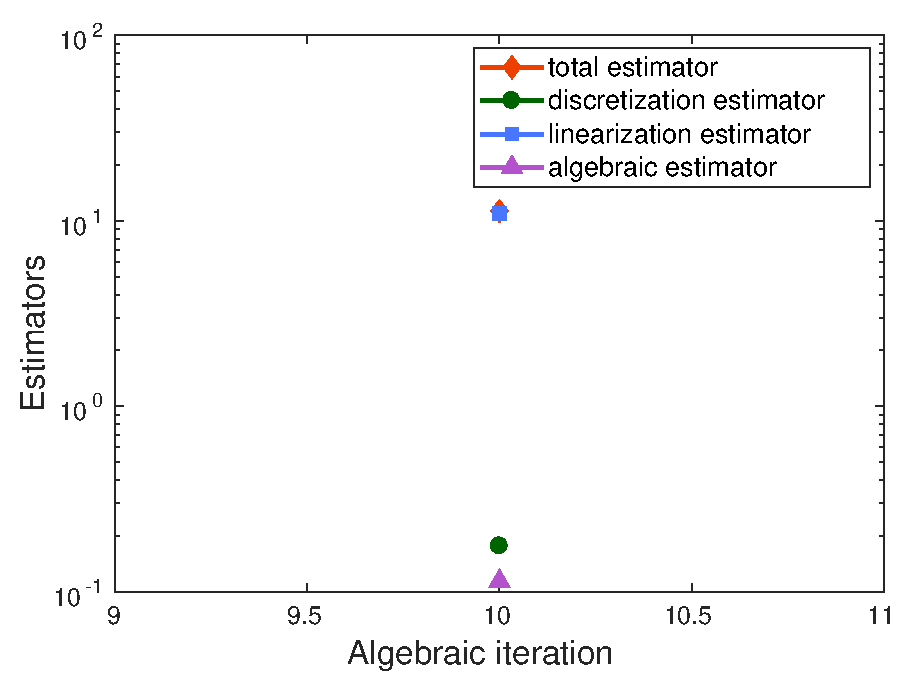
\includegraphics[width=0.50\textwidth]{fig_article_chap_1/inexacte_resolution_Hmax_015_number_gmres_iter_inside_first_newton_step.eps} 
\end{figure}
\end{frame}
\begin{frame}
\frametitle{Newton-min adaptivity}
\hspace{2 cm} Exact/Adapt inexact Newton \hspace{3.5 cm } Inexact Newton\begin{figure}
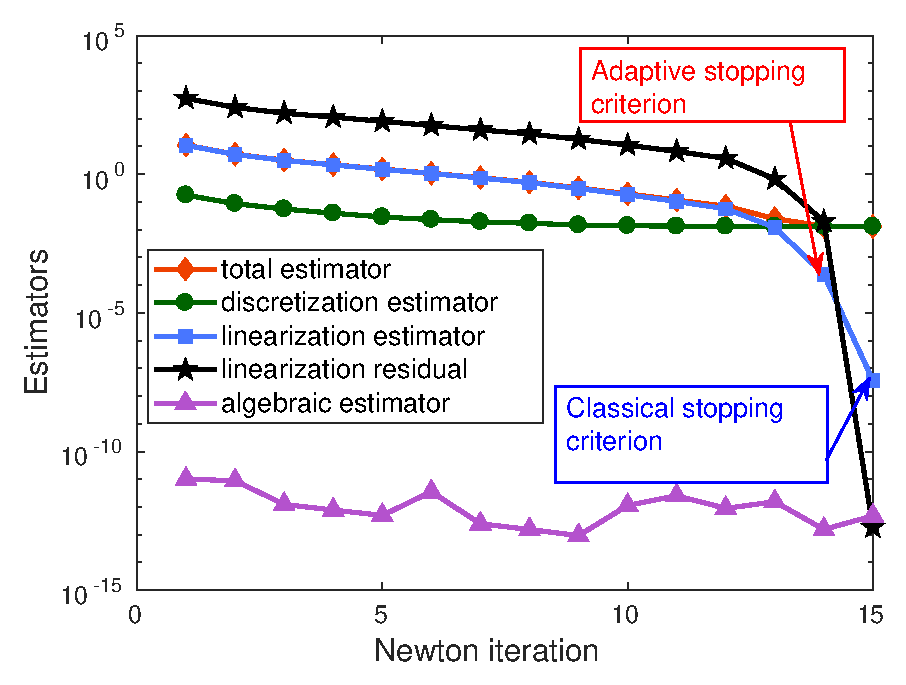
\includegraphics[width=0.5\textwidth]{fig_article_chap_1/exact_adapt_resolution_estimators_newton_iter_Hmax_015.eps}    
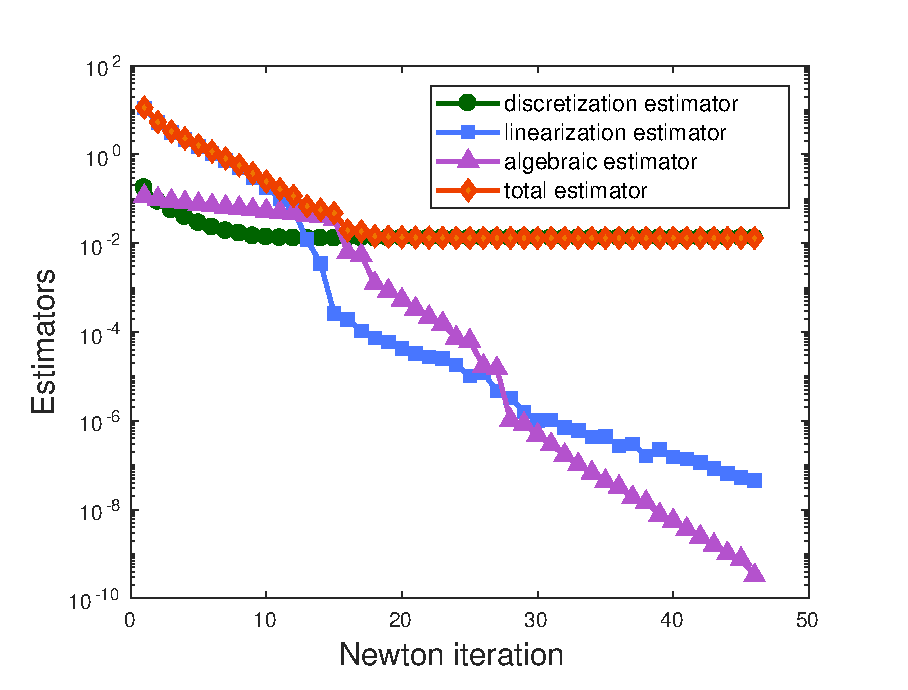
\includegraphics[width=0.5\textwidth]{fig_article_chap_1/inexacte_resolution_Hmax_015_estimators_newton_step.eps}     
\end{figure}
\end{frame}

\begin{frame}
\frametitle{Overall performance}
\begin{figure}
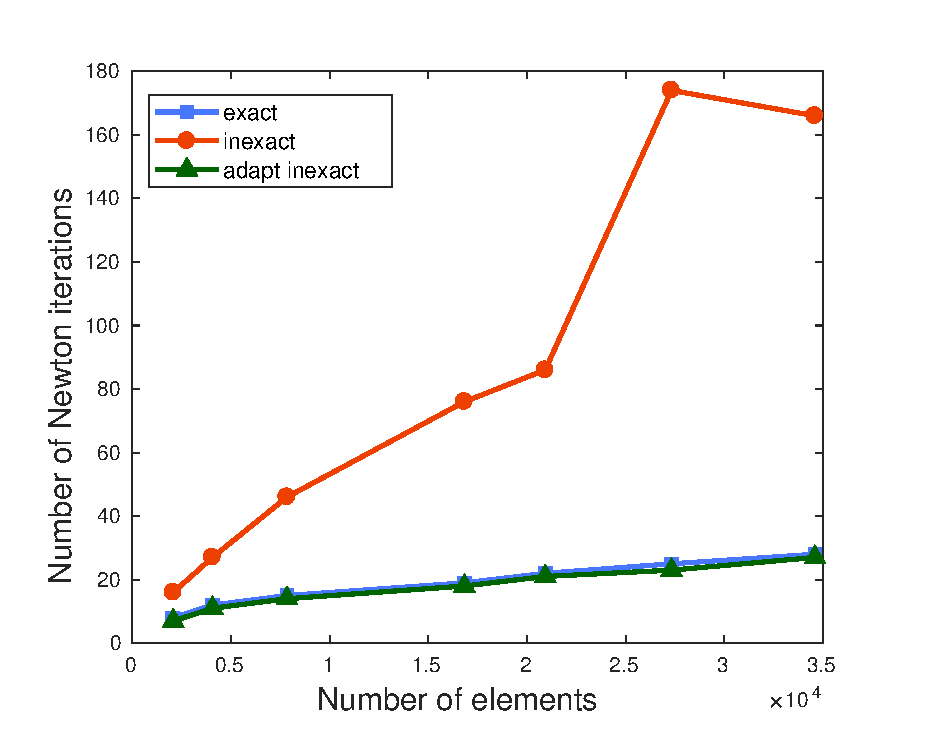
\includegraphics[width=0.47\textwidth]{fig_article_chap_1/comparison_three_methods_number_Newton_iter_number_elements.eps}  \quad  
 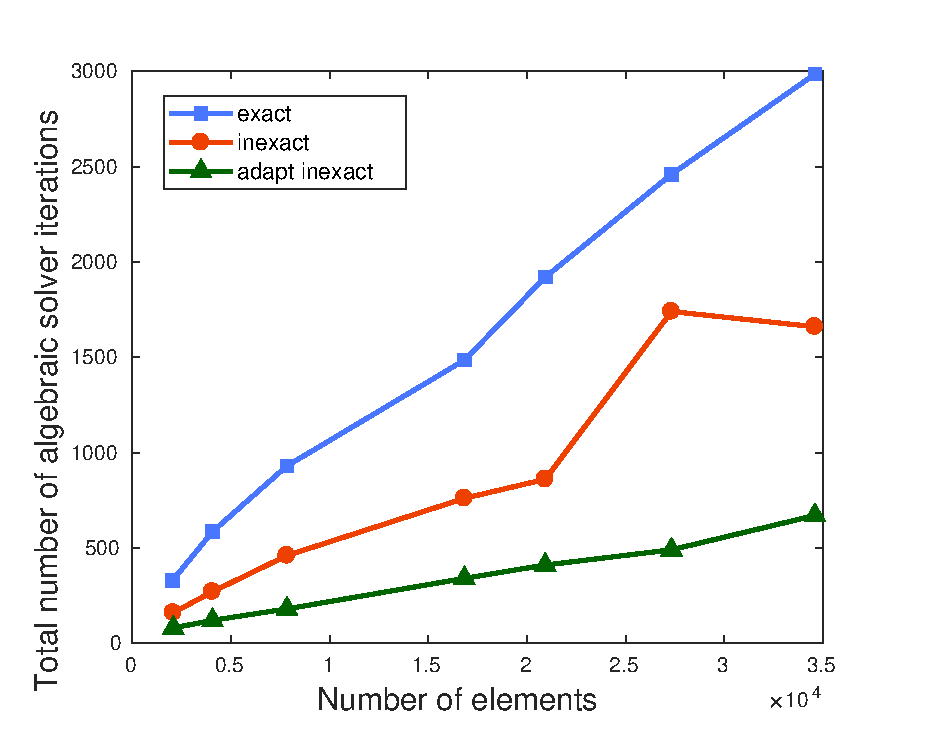
\includegraphics[width=0.50\textwidth]{fig_article_chap_1/comparison_three_methods_total_number_Newton_Gmres_iter_number_elements.eps}     
\end{figure}
\end{frame}


\begin{frame}
\frametitle{Effectivity indices}
\begin{figure}
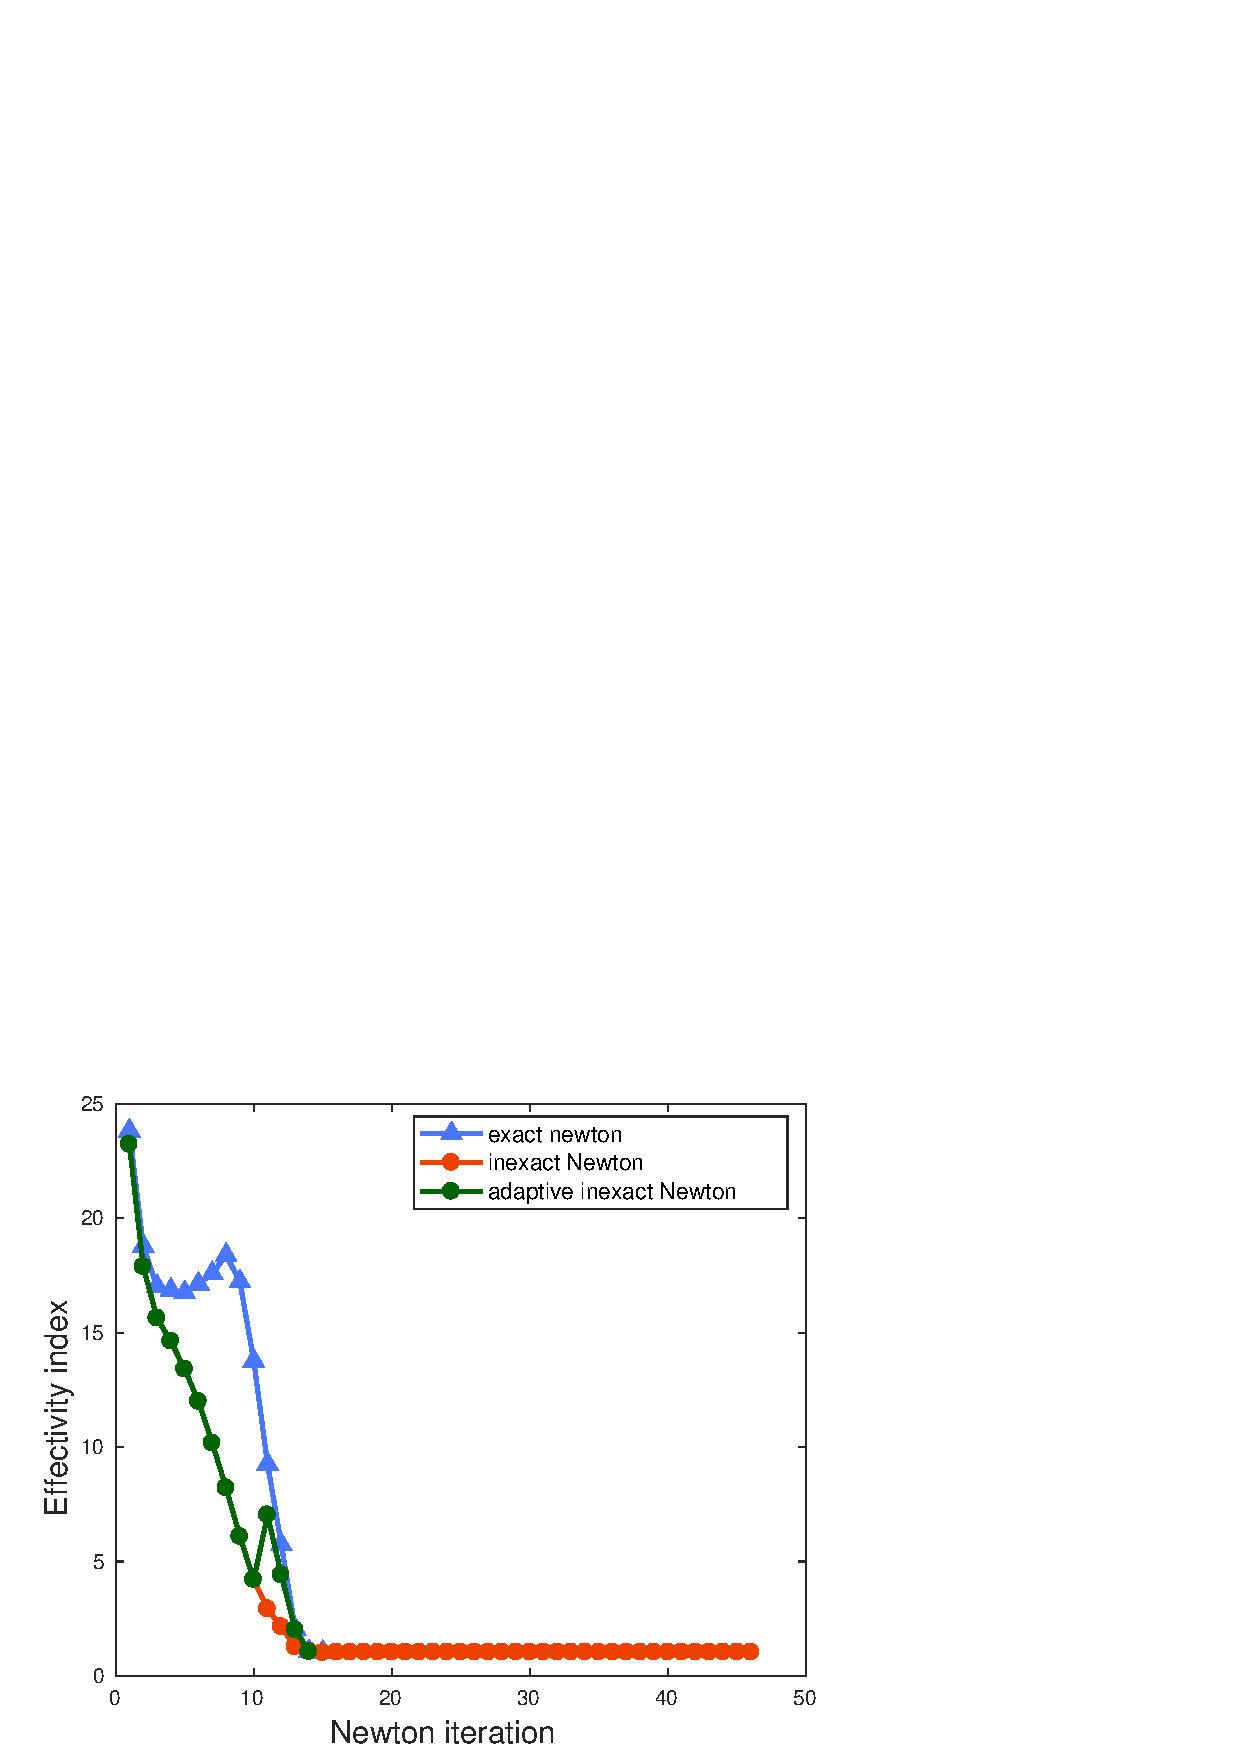
\includegraphics[width=0.47 \textwidth]{fig_article_chap_1/effectivity_index_3_methods_Hmax_015.pdf}   \quad 
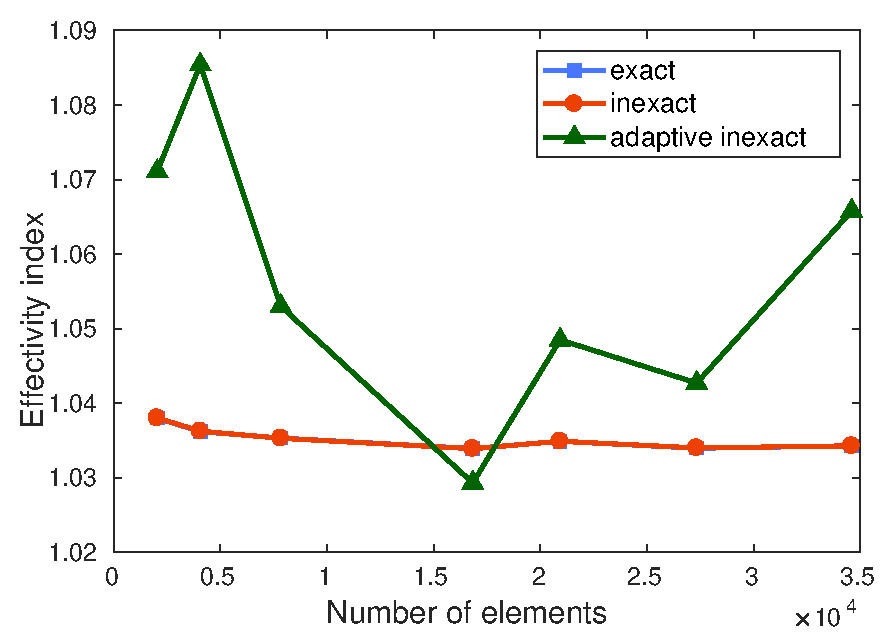
\includegraphics[width=0.50\textwidth]{fig_article_chap_1/effectivity_index_3_methods_number_elements.eps}     
\end{figure}
\end{frame}
\begin{frame}
 \hspace{1 cm}\textcolor{red}{\textbf{Local distribution of the error}} \hspace{2.5 cm}    \textcolor{red}{\textbf{Local error estimator}}
\begin{figure}
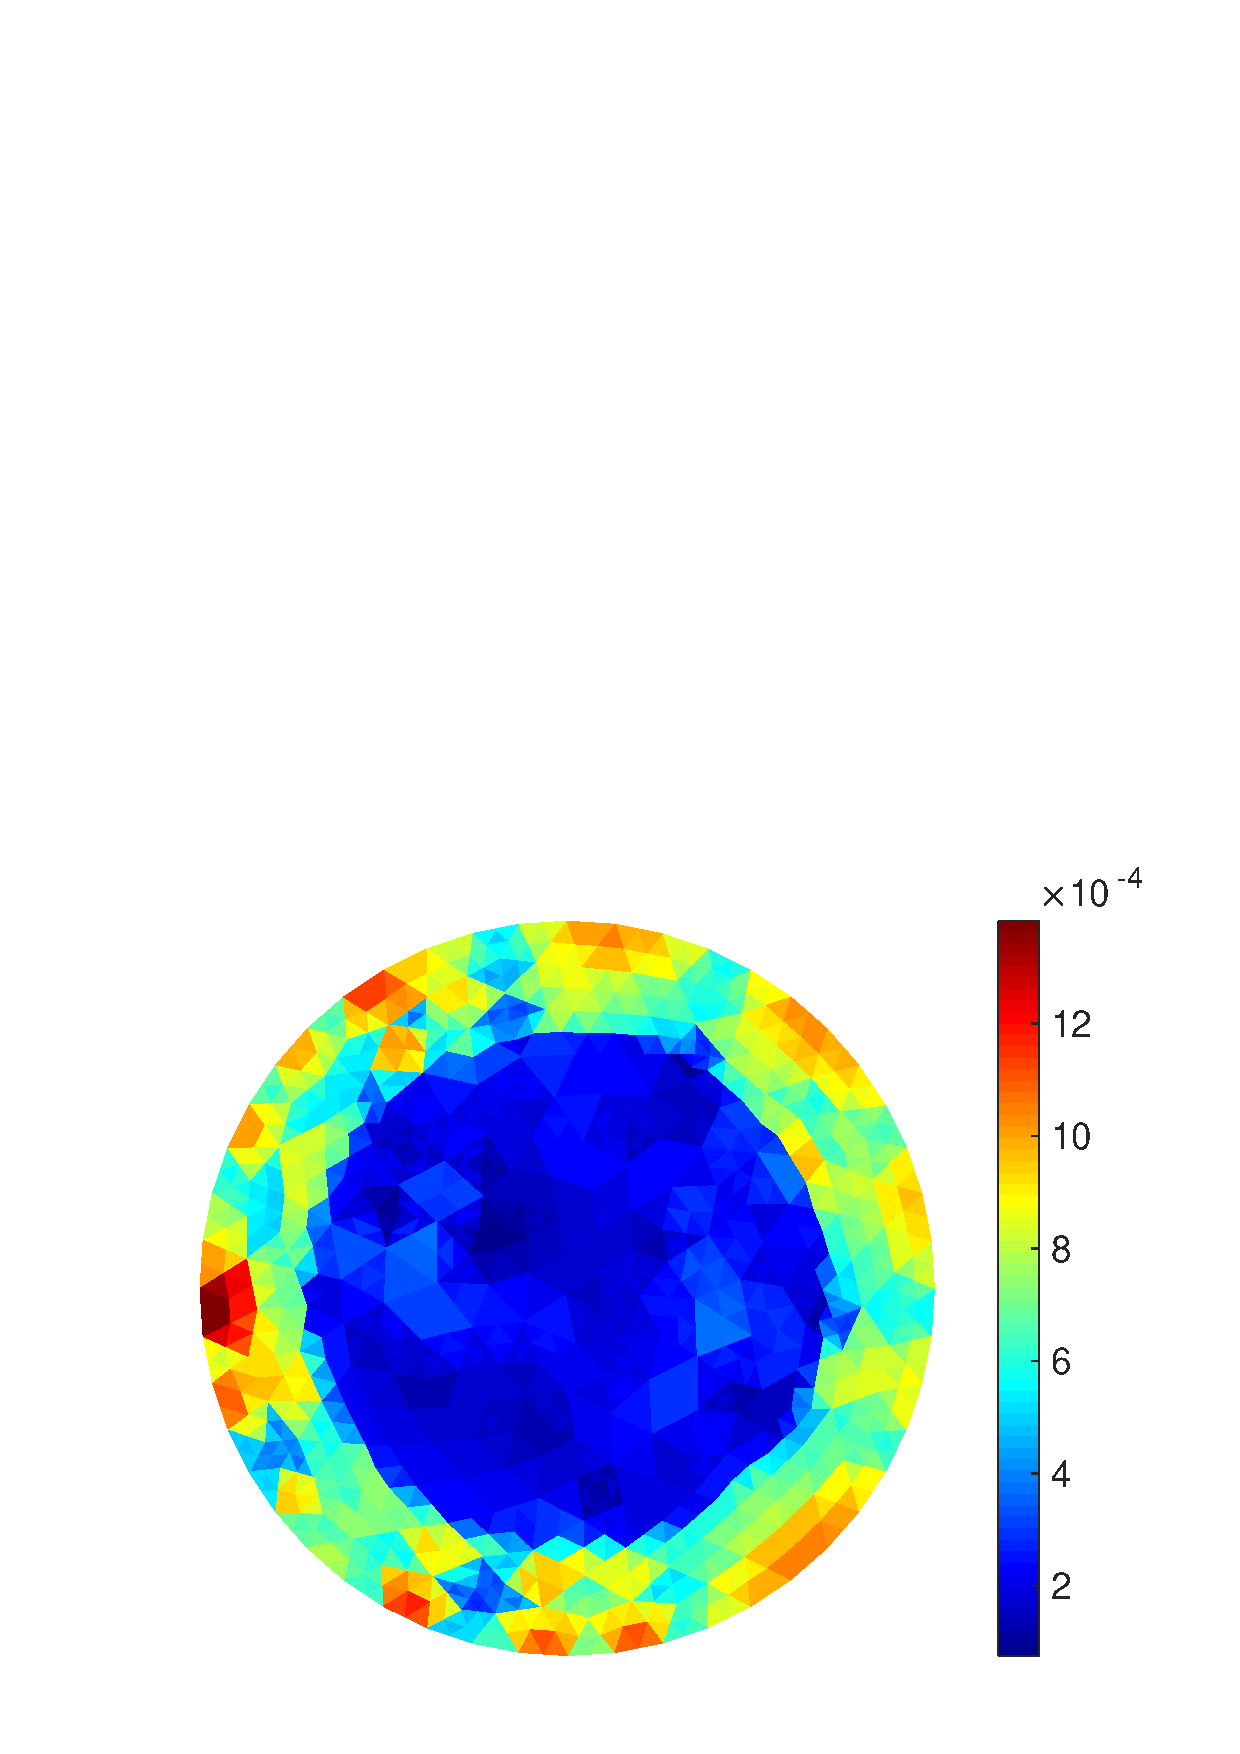
\includegraphics[width=0.47 \textwidth]{fig_article_chap_1/energy_norm_second_level_inexact_newton_iter_30.pdf}  
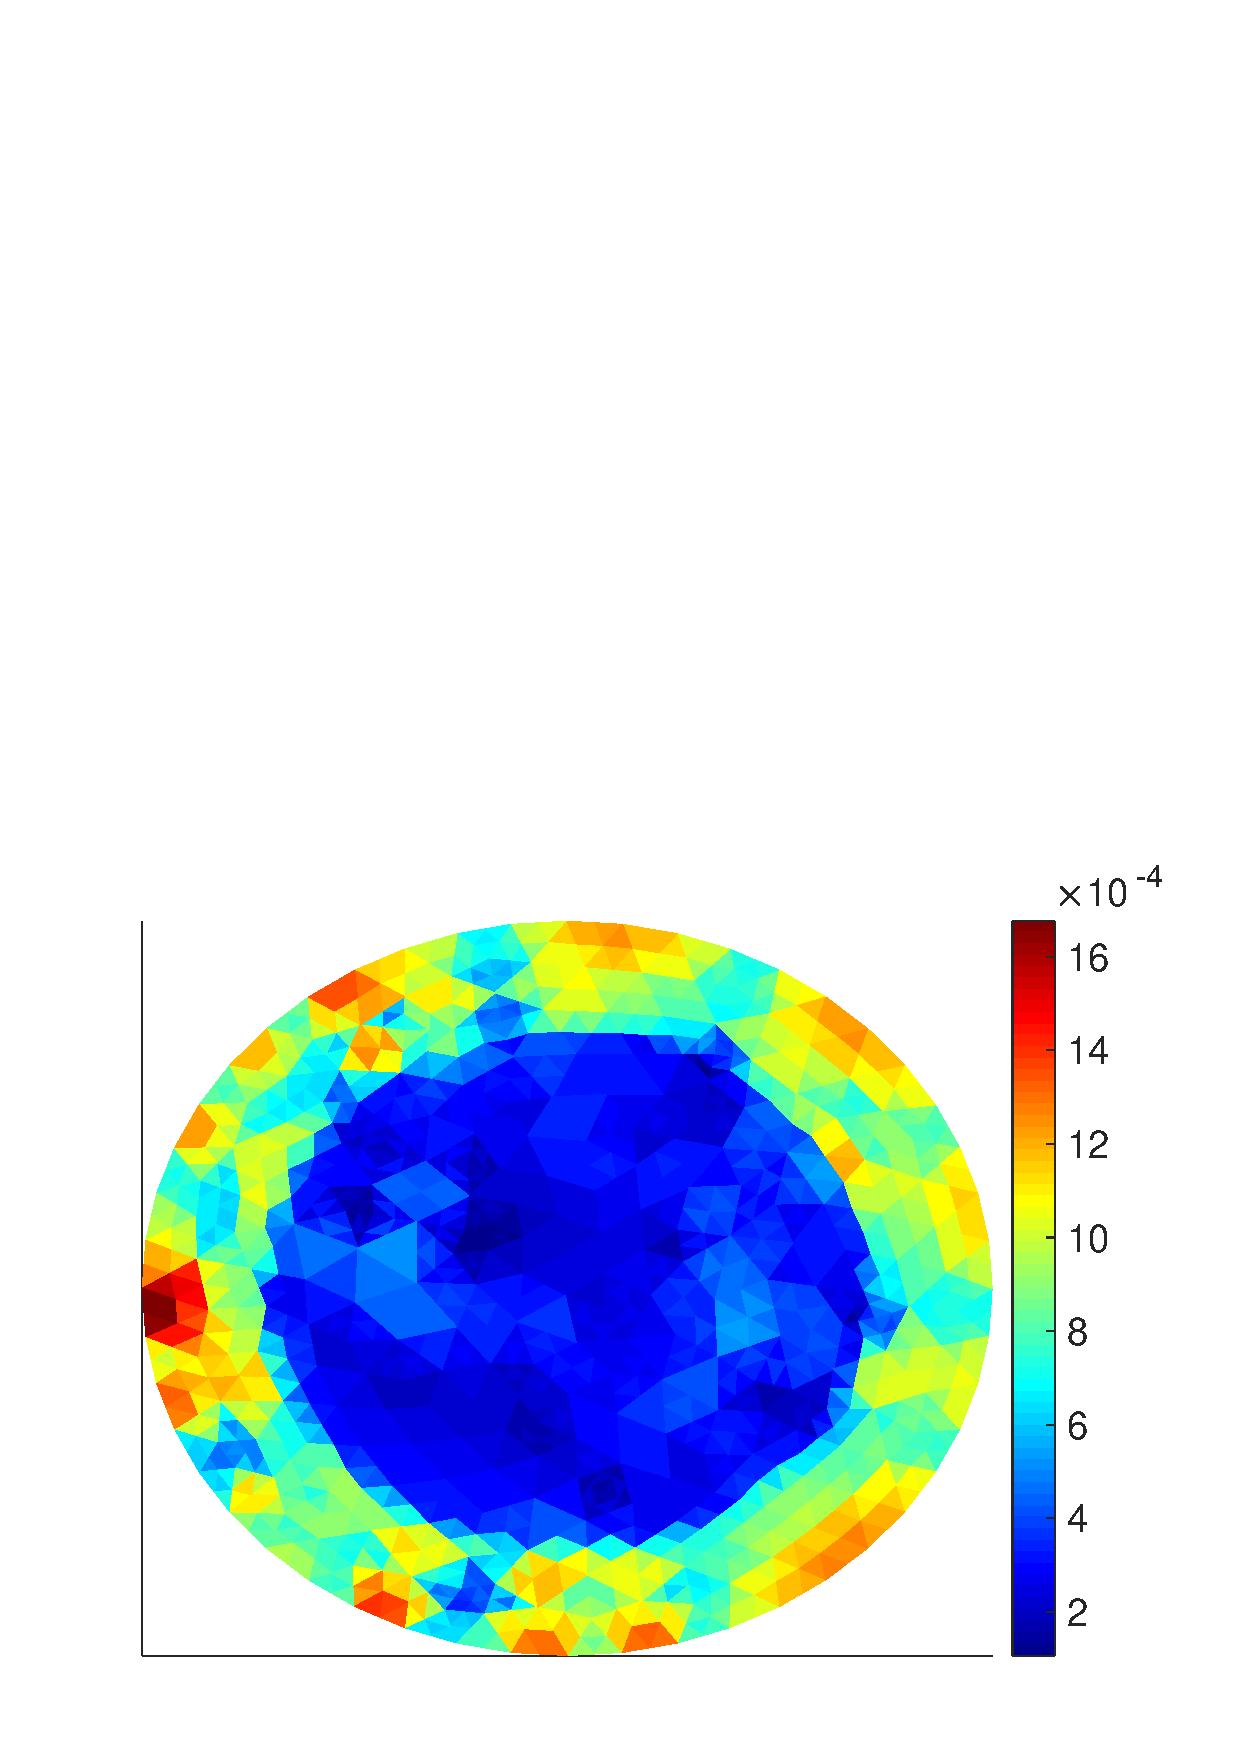
\includegraphics[width=0.48 \textwidth]{fig_article_chap_1/estimator_actual_error_inexact_newton_iter_30second_level.pdf} 
\end{figure}
\end{frame}

\begin{frame}
\hspace{5 cm}
\textcolor{red}{\textbf{Contact estimator}}
\begin{figure}
\includegraphics[width=0.6 \textwidth]{fig_article_chap_1/modif_fig_contact_estimator_hmax0,09_Dt0,001_tt180}  
\end{figure}
\end{frame}
%
%%%
%%%
%%%
\section{Two-phase compositional flow}
\subsection{}
\begin{frame}
\frametitle{Model problem for the storage of radioactive wastes }
\vspace*{-0.6 cm}
\begin{equation*}
\dps
\left\lbrace\begin{array}{llccc}
\dps \partial_t l_\componentw(\textcolor{cadmiumgreen}{\Sl}) + \nab \cdot {\bm \Phi}_{\mathrm{w}}(\textcolor{cadmiumgreen}{\Sl,\Pl,\chihl}) = Q_{\componentw}, \\
\dps \partial_t l_\componenth(\textcolor{cadmiumgreen}{\Sl,\Pl,\chihl})  + \nab \cdot {\bm \Phi}_{\mathrm{h}}(\textcolor{cadmiumgreen}{\Sl,\Pl,\chihl})=\Qh,\\
\textcolor{electricpurple}{1 - \Sl} \geq 0, \;  \textcolor{carmine}{H\left(\Pl + \Pcp(\Sl) \right) - \beta_{\phasel} \chihl} \geq 0, \; \left(\textcolor{electricpurple}{1 - \Sl} \right) \cdot \left(\textcolor{carmine}{H\left(\Pl + \Pcp(\Sl) \right) - \beta_{\phasel} \chihl}\right)=0  
\end{array}
\right.
\end{equation*}
\begin{figure}
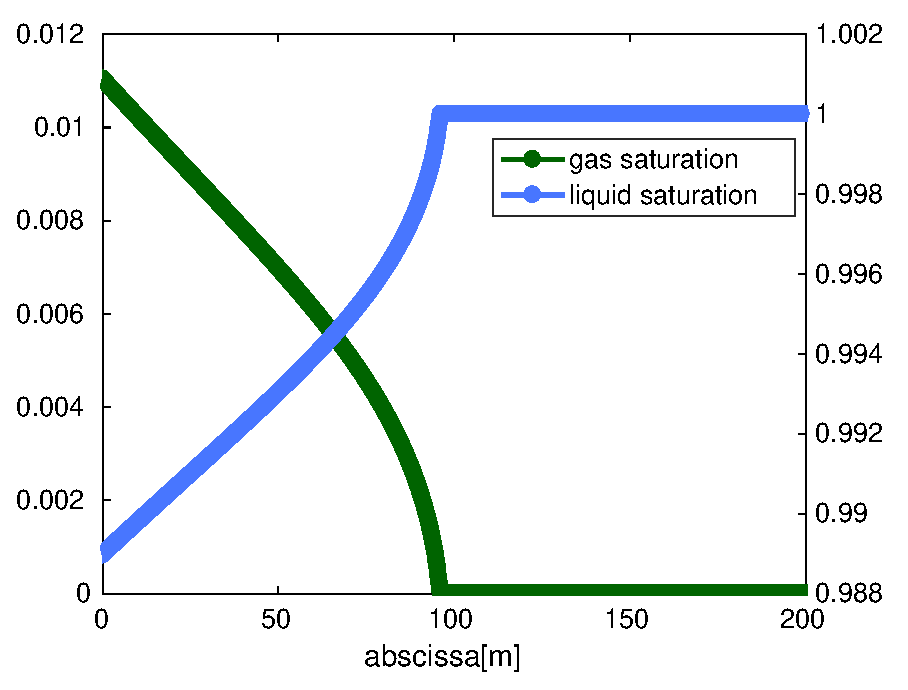
\includegraphics[width=0.45\textwidth]{fig_article_chap_3/saturations_cv_solver_1000_cells_nt=20} \qquad
\includegraphics[width=0.35\textwidth]{fig_article_chap_3/stockage_dechets_radioactifs_sans_texte}
\end{figure}

\end{frame}
%
%% DISCRETIZATION FINITE VOLUME
% \begin{frame}
% \frametitle{Discretization by the finite volume method}
% \textcolor{blue}{\textbf{Numerical solution: }}
% \begin{equation*}
% \bUn \egaldef (\bUn_K)_{K\in \Th}, \qquad \bUn_K \egaldef  (\SKn,\PKn,\chiKn) \quad \textcolor{cadmiumgreen}{\textbf{one value per cell and time step}} 
% \label{eq:finite:volume:approx}
% \end{equation*}
% \textcolor{cadmiumgreen}{\textbf{Time discretization:}}
% \\
%  \begin{figure}[htbp]
% \vspace{-0.6 cm}
%  \centering
%  \begin{picture}(200,60)(0,0)
%  \thicklines
%  \put(0,15){\line(200,0){200}}
%  %\put(0,10){\red{\line(0,10){10}}}
%  \put(0,0){\makebox(0,0){\small \red{$t_0 = 0$}}}
%  \put(0,15){\black{\circle*{6}}}
%  \put(25,10){\red{\line(0,10){10}}}
%  \put(25,0){\makebox(0,0){\small \red{$t_1$}}}
%  %\put(25,15){\blue{\circle*{6}}}
%  \put(12.5,30){\makebox(0,0){\small  \blue{$I_1$}}}
%  \put(50,10){\red{\line(0,10){10}}}
%  \put(50,0){\makebox(0,0){\small \red{$t_2$}}}
%  %\put(75,15){\blue{\circle*{6}}}
%  \put(37.5,30){\makebox(0,0){\small  \blue{$I_2$}}}
%  \put(75,30){\makebox(0,0){\small \blue{$\cdots$}}}
%  \put(75,0){\makebox(0,0){\small \red{$\cdots$}}}
%  \put(112.5,30){\makebox(0,0){\small \blue{$I_{n}$}}}
%  %\put(215,15){\blue{\circle*{6}}}
%  \put(100,10){\red{\line(0,10){10}}}
%  \put(100,0){\makebox(0,0){\red{\small $t_{n-1}$}}}
%  \put(125,10){\red{\line(0,10){10}}}
%  \put(125,0){\makebox(0,0){\red{\small $t_{n}$}}}
%  \put(150,30){\makebox(0,0){\small \blue{$\cdots$}}}
%  \put(150,0){\makebox(0,0){\small \red{$\cdots$}}}
%  \put(175,0){\makebox(0,0){\small \red{$t_{\Nt - 1}$}}}
%  \put(175,10){\red{\line(0,10){10}}}
%  %\put(355,15){\blue{\circle*{6}}}
%  \put(187.5,30){\makebox(0,0){\small \blue{$I_{\Nt}$}}}
%  \put(200,0){\makebox(0,0){\small \red{$t_{\Nt} = t_{\mathrm{F}}$}}}
%  %\put(240,10){\red{\line(0,10){10}}}
%  \put(200,15){\black{\circle*{6}}}
%  \end{picture}
% \qquad \qquad
% \includegraphics[scale = 0.5]{fig_article_chap_2/approx_time_derivative.pdf}
%  \end{figure}
% \begin{minipage}[c]{0.3 \textwidth}
% \textcolor{cadmiumgreen}{\textbf{Space discretization:}} $\Th$ a superadmissible family of conforming simplicial meshes of $\Omega$. \textcolor{blue}{Number of cells : $\Nsp$}
% \begin{equation*}
% \dps 
% \left(\nab v \cdot \bn_{K,\sigma},1\right)_{\sigma} := \dps |\sigma| \frac{v_L - v_K}{d_{KL}} \hspace{0.2 cm} \sigma = \overline{K} \cap \overline{L},
% \end{equation*}
% \end{minipage}
% \hfill
% \begin{minipage}[c]{0.5 \textwidth}
% \begin{figure}
% \includegraphics[width = 0.7 \textwidth]{fig_article_chap_3/gradient_discretization.pdf}
% \end{figure}
% \end{minipage}
% \end{frame}

\begin{frame}
\frametitle{Discretization by the finite volume method}
\textcolor{cadmiumgreen}{\textbf{Numerical solution: }}
\begin{equation*}
 \bUn \egaldef (\bUn_K)_{K\in \Th}, \qquad \bUn_K \egaldef  (\SKn,\PKn,\chiKn) \quad \textcolor{cadmiumgreen}{\textbf{one value per cell and time step}} 
\end{equation*}
\textcolor{blue}{\textbf{Discretization of the water equation}}
\begin{equation*}
S_{\mathrm{w},K}^n(\bU^n) \egaldef |K| \partial_t^n \lwK  + \sum_{\sigma \in \EK} {F}_{\componentw,K,\sigma}(\bU^{n})- |K|\QwKn = 0,
\end{equation*}
% \begin{equation*}
% {F}_{\componentw,K,\sigma}(\bUn) \egaldef \rhowl (\mobilityliq)_{\sigma}^{n} (\psil)_{\sigma}^{n} - (\jhl)_{\sigma}^{n} \quad \sigma \in \EKint \quad \overline{\sigma} = \overline{K} \cap \overline{L}.
% \end{equation*}
\invisible<1>{
\textcolor{blue}{\textbf{Discretization of the hydrogen equation}}
\begin{equation*} 
S_{\mathrm{h},K}^{n}(\bU^n)\egaldef |K| \partial_t^n \lhK + \sum_{\sigma \in \EK} {F}_{\componenth,K,\sigma}(\bUn) - |K| \QhKn = 0,
\end{equation*}
% \begin{equation*}
%  {F}_{\componenth,K,\sigma}(\bUn) \egaldef \betal \chisigman (\mobilityliq)_{\sigma}^{n} (\psil)_{\sigma}^{n} + (\psig)_{\sigma}^{n} (\mobilitygas)_{\sigma}^{n} (\rhog)_{\sigma}^{n} + (\jhl)_{\sigma}^{n} , \quad \sigma \in \EKint \quad \overline{\sigma} = \overline{K} \cap \overline{L}.
% \end{equation*}
\invisible<2>{
At each time step, for each components, we obtain the nonlinear system of algebraic equations
\begin{equation*}
S_{c,K}^n(\bU_h^n)=0
\end{equation*}
\invisible<3>{
}}}
\end{frame}
%
\begin{frame}
\frametitle{Discrete complementarity problem and semismoothness}
\textcolor{red}{\textbf{Discretization of the nonlinear complementarity constraints}}
\begin{equation*}
\textcolor{electricpurple}{\mathcal{K}(\bU_K^n)} \egaldef \textcolor{electricpurple}{1-\SKn} \quad \textcolor{carmine} {\mathcal{G}(\bU_K^n)} \egaldef  \textcolor{carmine}{H(\PKn\hspace{-0.05 cm}+\hspace{-0.05 cm}\Pcp(\SKn))-\betal \chiKn}
\end{equation*}
\pause
The discretization reads
\begin{equation*}
\begin{split}
&S_{c,K}^n(\bU_h^n)=0\\
& \textcolor{electricpurple}{\mathcal{K}(\bU_K^n)} \geq 0, \quad   \textcolor{electricpurple}{\mathcal{G}(\bU_K^n)} \geq 0, \quad \textcolor{electricpurple}{\mathcal{K}(\bU_K^n)} \cdot \textcolor{electricpurple}{\mathcal{G}(\bU_K^n)}=0
\end{split}
\end{equation*}
\pause
\begin{itemize}
\item
\textcolor{cadmiumgreen}{\textbf{We reformulate the complementarity constraints with C-functions}}
\item
\textcolor{cadmiumgreen}{\textbf{We employ inexact semismooth linearization}}
\item
\textcolor{cadmiumgreen}{\textbf{Can we estimate each error component?}}
\end{itemize}
\end{frame} 
%
\begin{frame}
\centering
\Huge{\textcolor{carmine}{A posteriori error estimates}}
\end{frame}
%
\begin{frame}
\frametitle{Weak solution}
\vspace{-0.2 cm}
\textcolor{cadmiumgreen}{\textbf{Motivation: Define rigorously the dual norm of the residual}}
\vspace*{-0.1 cm}
 \begin{equation*}
\left\|\mathcal{R}_{\componentc}(\Shtaunki,\Phtaunki,\chihtaunki) \right\|_{\Xn'} \egaldef \sup_{\substack{\varphi \in \Xn \\ \left\|\varphi\right\|_{\Xn} = 1}}  \int_{\In} 
 \left(\Qc - \partial_t \lchtaunki , \varphi\right)_{\Omega}(t) + \left(\Phichtaunki,\nab \varphi \right)_{\Omega}(t)\,\mathrm{dt} 
 \end{equation*}
\vspace{-0.1 cm}
\pause
\begin{equation*}
\begin{split}
&X \egaldef L^2((0,\tF);H^1(\Omega)), \ Y  \egaldef H^1((0,\tF);L^2(\Omega)), 
%\ \widehat{Y} \egaldef H^1((0,\tF);L^{\infty}(\Omega)),\\
 \  Z \egaldef L_{+}^2((0,\tF);L^{\infty}(\Omega)) \\& \left\| \varphi \right\|_{X_n} \egaldef \int_{\In} \sum_{K \in \Th} \left\| \varphi \right\|_{X,K}^2 \mathrm{dt}, \hspace{0.15 cm} \left\| \varphi \right\|_{X,K}^2 \egaldef \varepsilon h_K^{-2} \left\|\varphi\right\|_K^2 + \left\|\nab \varphi\right\|_K^2
\end{split}
\end{equation*}
\pause
\textcolor{blue}{\textbf{Assumption:}}
\begin{itemize}
\item
% $\Sl \in \widehat{Y}$, \ 
$\textcolor{electricpurple}{1-\Sl} \in Z$, \ $\lc \in Y$, \ $\Pl \in X$, \ $\chihl \in X$, \ $\Phic \in L^2((0,\tF); \HdivOmeg)$
\item 
$\dps \int_{0}^{\tF} \left(\partial_t \lc, \varphi \right)_{\Omega}(t)\,\mathrm{dt}-\hspace{-0.1 cm}\int_{0}^{\tF} \left(\Phic, \nab \varphi \right)_{\Omega}(t)\,\mathrm{dt} = \hspace{-0.1 cm} \int_{0}^{\tF} \left(\Qc, \varphi \right)_{\Omega}(t)\,\mathrm{dt} \quad \forall \varphi \in X$
\item 
$\dps \int_{0}^{\tF} \left(\lambda - \left(\textcolor{electricpurple}{1 - \Sl}\right), \textcolor{carmine}{H[\Pl+\Pcp(\Sl)]-\betal \chihl}  \right)_{\Omega}(t)\,\mathrm{dt} \geq 0 \quad \forall \lambda \in Z$
\item
the initial condition  holds
\end{itemize}
\end{frame}
% %
\begin{frame}
\frametitle{Approximate solution}
\vspace{-0.4 cm}
\begin{equation*}
\SKnki \in \textcolor{cadmiumgreen}{\PzerodTh} \quad \PKnki \in \textcolor{cadmiumgreen}{\PzerodTh} \quad \chiKnki \in \textcolor{cadmiumgreen}{\PzerodTh}
\end{equation*}
The discrete liquid pressure and discrete molar fraction do not belong to $H^1(\Omega)$
\invisible<1>{
\textcolor{blue}{\textbf{We construct a conforming solution:}}
\begin{figure}
\centering
\includegraphics[width = 0.6 \textwidth]{fig_article_chap_3/image_oswald}
\end{figure}
\invisible<2>{
Space-time functions:
\begin{equation*}
\Shtaunki  \in \textcolor{cadmiumgreen}{Y}, \quad  \Phtaunki \in \textcolor{cadmiumgreen}{\PtwodTh} \ \textcolor{red}{\bm \notin} \ X, \quad \chihtaunki \in \textcolor{cadmiumgreen}{\PtwodTh} \ \textcolor{red}{\bm \notin} \ X
\end{equation*}
\vspace{-0.2 cm}
\begin{equation*}
  \begin{split}
& \tildePhtaunki \in \textcolor{cadmiumgreen}{\PtwocTh} \ \textcolor{red}{\bm \in} \ X,\\
& \tildechihtaunki \in \textcolor{cadmiumgreen}{\PtwocTh} \textcolor{red}{\bm \in} X.
\end{split}
\end{equation*}
\invisible<3>{
}}}
\end{frame}

\begin{frame}
\frametitle{Error measure}
\vspace{-0.3 cm}
\begin{itemize}
\item 
\textcolor{cadmiumgreen}{\textbf{Dual norm of the residual for the components}}
\pause
\item
\textcolor{cadmiumgreen}{\textbf{Residual for the constraints}}
\begin{equation*}
  \mathcal{R}_{\mathrm{e}}(\Shtaunki,\Phtaunki,\chihtaunki) \egaldef \int_{\In}\left(\textcolor{electricpurple}{1 - \Shtaunki}, \textcolor{carmine}{H \left[\Phtaunki + \Pcp(\Shtaunki)\right] - \betal \chihtaunki} \right)_{\Omega}(t)\,\mathrm{dt}
\end{equation*}
\pause
\item
\textcolor{cadmiumgreen}{\textbf{Error measure for the nonconformity of the pressure}} $\mathcal{N}_{P}(\Phtaunki)$
\pause
\item \textcolor{cadmiumgreen}{\textbf{Error measure for nonconformity of the molar fraction}} $\mathcal{N}_{\chi}(\chihtaunki)$
\end{itemize}
\begin{equation*}
\mathcal{N}^{n,\kk,\ii}  \egaldef \left\{\sum_{\componentc \in\mathcal{C}} \left\|\mathcal{R}_{\componentc}(\Shtaunki,\Phtaunki,\chihtaunki) \right\|_{X_n'}^2 \right\}^{\frac{1}{2}} + \left\{\sum_{\phasep \in \mathcal{P}}\mathcal{N}_{\phasep}^2 + \mathcal{N}_{\chi}^2\right\}^{\frac{1}{2}} + \mathcal{R}_{\mathrm{e}}(\Shtaunki,\Phtaunki,\chihtaunki)
\end{equation*}
\begin{theorem}
\begin{equation*}
\mathcal{N}^{n,\kk,\ii} \leq \etadiscnki + \etalinnki + \etaalgnki
\end{equation*} 
\end{theorem}
\textcolor{red}{\textbf{How do we construct each error estimators?}}
\end{frame}
%
\begin{frame}
\frametitle{Component flux reconstructions}
\vspace{-0.1 cm}
\textcolor{cadmiumgreen}{\textbf{The finite volume scheme provides}}
\begin{equation*} 
  |K| \partial_t^n \lcK + \sum_{\sigma \in \EK} {F}_{\componentc,K,\sigma}(\bUn) =  |K|\QcKn
\end{equation*}
\invisible<1>{
\vspace{-0.1 cm}
\textcolor{cadmiumgreen}{\textbf{Inexact semismooth linearization}}

\begin{equation*}
\label{eq:flux:equation}
 \frac{|K|}{\Delta t}\left[\lcK\left(\bU^{n,\kk-1}\right) - \lcK^{n-1} + \mathcal{L}_{\componentc,K}^{n,\kk,\ii}\right] + \sum_{\sigma \in \EKint} \mathcal{F}_{\componentc,K,\sigma}^{n,\kk,\ii}- |K|\QcKn + {\bR}_{\componentc,K}^{n,\kk,\ii} = 0
\end{equation*}
\vspace{-0.1 cm}
\invisible<2>{
 \textcolor{blue}{Linear perturbation in the accumulation}
\begin{equation*}
\mathcal{L}_{\componentc,K}^{n,\kk,\ii} \egaldef \sum_{K' \in \Th} \frac{|K|}{\Delta t}  \frac{\partial \lcK^n}{\partial \bU_{K'}^n}(\bU_{K'}^{n,\kk-1}) \left[\bU_{K'}^{n,\kk,\ii}-\bU_{K'}^{n,\kk-1} \right]
\end{equation*}
\textcolor{blue}{Linearized component flux}
\begin{equation*}
\label{eq:linearized:semi:smooth:component:flux}
\mathcal{F}_{\componentc,K,\sigma}^{n,\kk,\ii} \egaldef \sum_{K' \in \Th} \frac{\partial {F}_{\componentc,K,\sigma}}{\partial \bU_{K'}^n} \left(\bU^{n,\kk-1}\right) \left[\bU_{K'}^{n,\kk,\ii} -\bU_{K'}^{n,\kk-1} \right] + {F}_{\componentc,K,\sigma}\left(\bU^{n,\kk-1}\right)
\end{equation*}
\invisible<3>{
}}}
\end{frame}
% 
 \begin{frame}
 \textcolor{cadmiumgreen}{\textbf{Discretization error flux reconstruction:}}
\begin{equation*}
\Thetachdiscnki|_{K} \in \RTzero(K) \quad \left(\Thetachdiscnki \cdot \bn_K,1 \right)_{\sigma} \egaldef F_{\componentc,K,\sigma}\left(\bU^{n,\kk, \ii}\right) \quad \forall K \in \Th
\end{equation*}
\invisible<1>{
 \textcolor{cadmiumgreen}{\textbf{Linearization error flux reconstruction:}}
\begin{equation*}
\Thetachlinnki|_{K} \in \RTzero(K) \quad \left(\Thetachlinnki \cdot \bn_K,1 \right)_{\sigma} \egaldef \mathcal{F}_{\componentc,K,\sigma}^{n,\kk,\ii} -  F_{\componentc,K,\sigma}\left(\bU^{n,\kk, \ii}\right) \quad \forall K \in \Th
\end{equation*}
\invisible<2>{
\textcolor{cadmiumgreen}{\textbf{Algebraic error flux reconstruction:}}
\begin{equation*}
\Thetachalgnkinu  \egaldef {\bm \Theta}_{\componentc,h,\mathrm{disc}}^{n,\kk,\ii+\nuu} + {\bm \Theta}_{\componentc,h,\mathrm{lin}}^{n,\kk,\ii+\nuu} - \left(\Thetachdiscnki + \Thetachlinnki \right)
 \quad \forall K \in \Th
\end{equation*}
\invisible<3>{
 \textcolor{red}{\textbf{Total flux reconstruction:}} 
\begin{equation*}
\Thetachnkinu \egaldef \Thetachdiscnki+\Thetachlinnki+\Thetachalgnkinu \ \textcolor{red}{\bm \in} \ \HdivOmeg
 \end{equation*}
\invisible<4>{
}}}}
 \end{frame}
%
\begin{frame}
\frametitle{Error estimators}
\textcolor{red}{Violation of physical properties of the approximate solution}
\begin{equation*}
\partial_t \lc + \nab \cdot \Thetachnkinu \neq \Qc \quad \Thetachnkinu \neq \Phichtaunki(t^n)
\end{equation*}
\textcolor{red}{Violation of the complementarity constraints}
\begin{equation*}
\textcolor{electricpurple}{1 - \Shtaunki} \ngeq 0 \quad \textcolor{carmine}{H\left[\Phtaunki + \Pcp\left(\Shtaunki\right)\right]-\betal \chihtaunki} \ngeq 0
\end{equation*}
\textcolor{red}{Nonconformity of the approximate solution}
\begin{equation*}
\Phtaunki \notin X \quad \chihtaunki \notin X
\end{equation*}
\pause
\begin{enumerate}
\item 
\textcolor{cadmiumgreen}{\textbf{Discretization estimator}}
\item
\textcolor{cadmiumgreen}{\textbf{Linearization estimator}}
\item
\textcolor{cadmiumgreen}{\textbf{Algebraic estimator}}
\end{enumerate}
\end{frame}
%
\begin{frame}
\centering
\Huge{\textcolor{carmine}{Numerical experiments}}
\end{frame}
% 
\begin{frame}
\frametitle{Numerical experiments}
$\Omega$:  one-dimensional core with length $L = 200 m$. 
\\
\vspace{0.2 cm}
\textbf{Semismooth solver:} Newton-min
\\
\vspace{0.2 cm}
\textbf{Iterative algebraic solver:} GMRES.
\\
\vspace{0.2 cm}
\textbf{Time step:} $\Delta t = 5000$ years, 
\\
\vspace{0.2 cm}
\textbf{Number of cells:} $\Nsp = 1000$, \\
\vspace{0.2 cm}
\textbf{Final simulation time:} $\tF = 5 \times 10^{5}$ years.
\\
\vspace{0.2 cm}
\begin{figure}
\includegraphics[width= 1 \textwidth]{fig_article_chap_3/num_exp_finite_vol}
\end{figure}

\end{frame}
% 
%% VIOLATION COMPLEMENTARITY CONSTRAINTS
% \begin{frame}
%  \frametitle{Violation of the complementarity constraints}
% \begin{figure}
% \centering
% 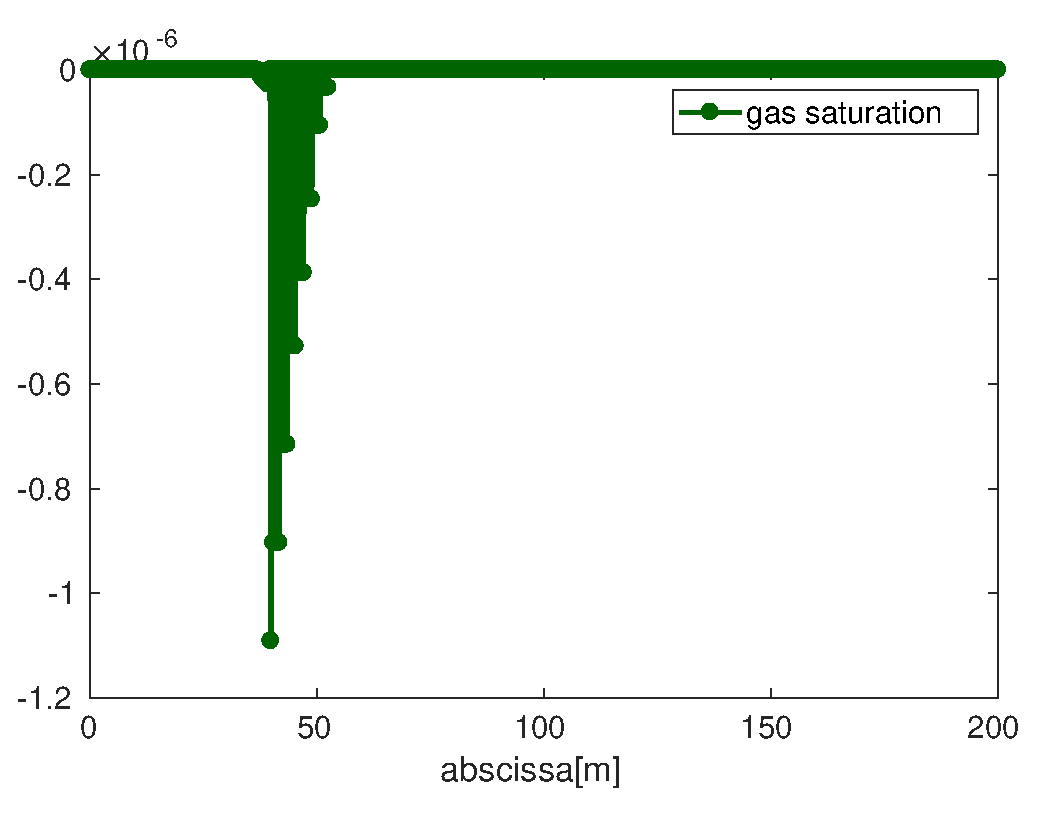
\includegraphics[width=0.45\textwidth]{fig_article_chap_3/gas_saturation_neg_gmres_iter2_newtoninter_4} \qquad
% \includegraphics[width=0.48\textwidth]{fig_article_chap_3/henry_constraint_neg_gmresiter2_newton_iter4}
% \end{figure}
% \end{frame}
%
\begin{frame}
\frametitle{Phase transition estimator}
\begin{figure}
  \begin{overprint}
    \onslide<1> \scriptsize{\textcolor{red}{\textbf{\bm{$t=2500$} years}}} 
\includegraphics[width=0.58\textwidth]{fig_article_chap_3/MODIF_phase_transition_estimator_appearance_gas_nt=inittime_cv}
    \onslide<2>
\scriptsize{\textcolor{red}{ \textbf{\bm{$t = 1.25 \times 10^4$} years}}}
\includegraphics[width=0.58\textwidth]{fig_article_chap_3/MODIF_phase_transition_estimator_appearance_gas_nt=2_cv}
    

\onslide<3>
\scriptsize{ \textbf{\textcolor{red}{ \bm{$t = 4.25 \times 10^4$} years}}}
\includegraphics[width=0.58\textwidth]{fig_article_chap_3/MODIF_phase_transition_estimator_appearance_gas_nt=9_cv}
    \end{overprint}
\end{figure}
\end{frame}
%
\begin{frame}
\frametitle{Overall performance $\gammalin = \gammaalg = 10^{-3}$}
\begin{figure}
\centering
\includegraphics[width=0.47\textwidth]{fig_article_chap_3/Cumulated_number_Newton_iterations_three_methods_Nx_1000}
\hspace{0.6 cm}
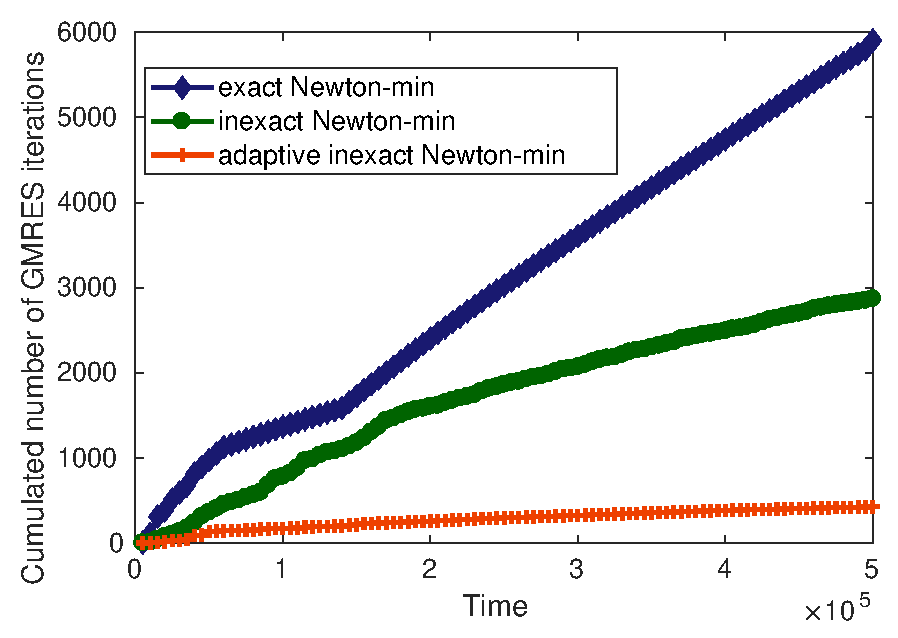
\includegraphics[width=0.47\textwidth]{fig_article_chap_3/Cumulated_number_gmres_iterations_three_methods_Nx_1000}
\end{figure}
\end{frame}
%
\begin{frame}
\frametitle{Accuracy  $\gammalin = \gammaalg = 10^{-3}$}
\vspace{-0.1 cm}
\textcolor{cadmiumgreen}{$t = 1.05 \times 10^5$ years \hspace{8 cm} $t = 3.5 \times 10^5$ years}
\begin{figure}
\centering
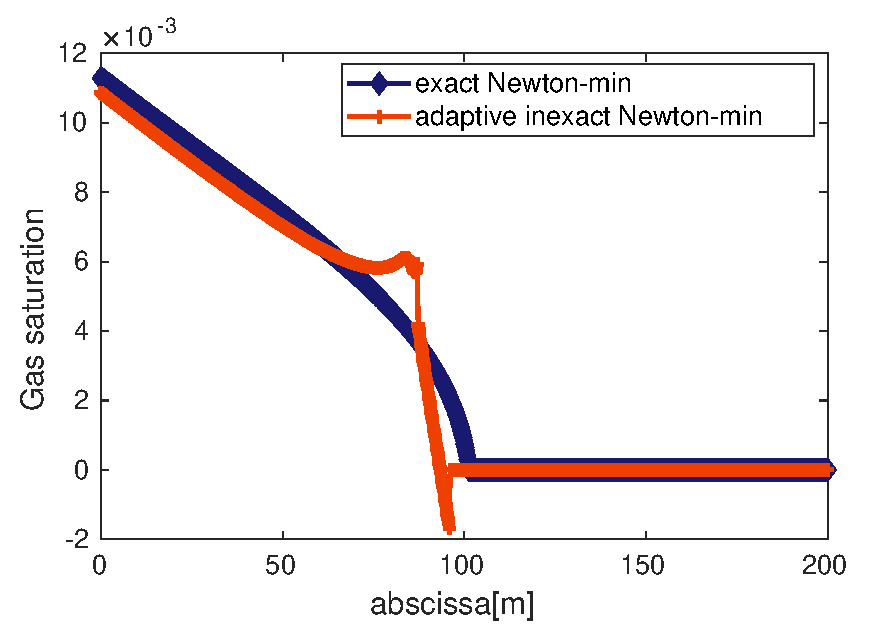
\includegraphics[width=0.48 \textwidth]{fig_article_chap_3/comparaison_plot_gas_saturations_exact_adapt_inexact_gamma_lin_gamma_alg_10-3_nt_21}
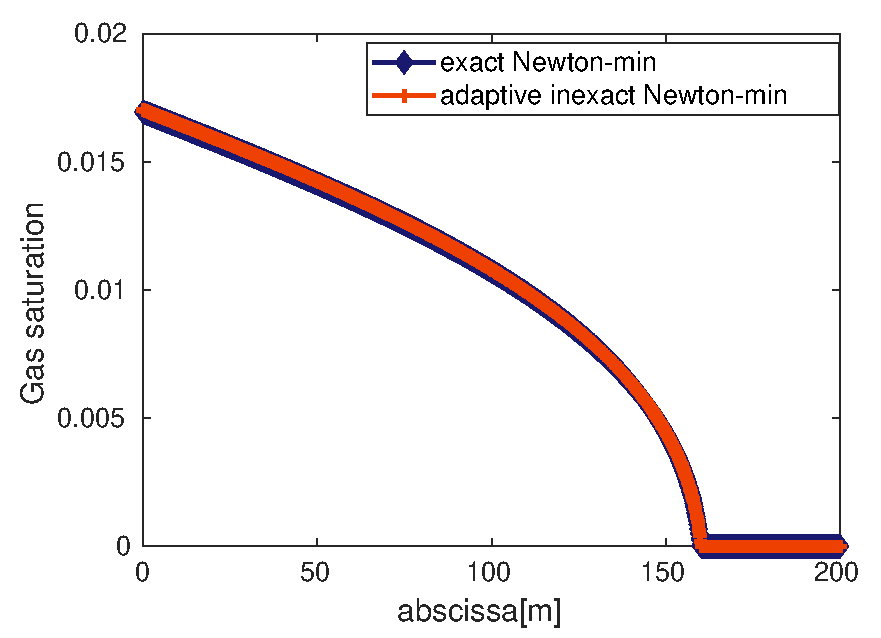
\includegraphics[width=0.48 \textwidth]{fig_article_chap_3/comparaison_plot_gas_saturations_exact_adapt_inexact_gamma_lin_gamma_alg_10-3_nt_70}
\end{figure}
\end{frame}
%
%% COMPLEMENTS NFB
% \begin{frame}
% \frametitle{Complements: Newton--Fischer--Burmeister}
% \vspace{-0.3 cm}
% \textcolor{cadmiumgreen}{
% \begin{equation*}
% \left[\fFB (\ba, \bb)\right]_l = \sqrt{\ba_l^2 + \bb_l^2} - (\ba_l + \bb_l) \quad l=1,\ldots,\Nsp.
% \end{equation*}
% }
% {\begin{table}
% \centering
% \begin{tabular}{lll}
% \hline\noalign{\smallskip}
% $\left(\gammaalg,\gammalin\right)$ & \hspace{-0.3 cm} \parbox{6.5 cm}{Cumulated number of Newton--Fischer--Burmeister iterations} &   \parbox{5 cm}{Cumulated number of GMRES  iterations}  \\
% \noalign{\smallskip}\hline\noalign{\smallskip}
% $\left(10^{-1},10^{-1} \right)$ & \qquad 100 & \quad \qquad 428 \\
% $\left(10^{-3},10^{-3}\right)$ & \qquad 119 & \quad \qquad 751 \\
% $\left(10^{-3},10^{-6}\right)$ & \qquad 482 & \quad \qquad 2074 \\
% $\left(10^{-6},10^{-3}\right)$ & \qquad 117 & \quad \qquad 1694 \\
% \textcolor{blue}{\textbf{Exact resolution}} & \qquad \textcolor{blue}{\textbf{757}} & \quad \hspace{0.2 cm} \quad \textcolor{blue}{\textbf{10089}} \\
% \noalign{\smallskip}\hline
% \end{tabular}
% \end{table}
% }

% \invisible<1>{
% \textcolor{red}{\textbf{Adaptive inexact resolution is faster than exact resolution. It saves roughly $90 \%$  of the iterations.}}
% \\
% \invisible<2>{
% \textcolor{red}{\textbf{Adaptive Newton-min is faster than Adaptive Newton--Fischer--Burmeister. It saves roughly $40 \%$ of the iterations.}}
% \invisible<3>{
% }}}
% \end{frame}
%
%
\section{Conclusion}
\subsection{}
\begin{frame}
\frametitle{Conclusion}
\begin{itemize}
\item
 Variational inequality: we devised a posteriori error estimates with $\Pp$ finite elements.
\item
 Two-phase flow with phase transition: a posteriori error estimates for a cell centered finite volume discretization. 
\item
Formulations with complementarity constraints and semismooth algorithms.
\item
 We distinguished the different error components.
\item Adaptive stopping criteria $\Rightarrow$ reduction of the number of iterations. 
\item
Extension of the stationary problem to a parabolic inequality:
\\
 \scriptsize{\textcolor{blue}{
 {\sc J.~Dabaghi, V.~Martin, and M.~Vohral{\'{\i}}k}, {\em A posteriori error estimate and adaptive stopping criteria for a parabolic variational inequality}. In preparation, 2019
 }}
\end{itemize}
\textcolor{cadmiumgreen}{\textbf{Implementation}}
\begin{itemize}
\item contact problem between two membranes: MATLAB code. Collaboration with Jan Pape{\v z} (INRIA Paris).
\item Two phase flow: MATLAB code. Collaboration with Ibtihel Ben Gharbia (IFPEN).
\end{itemize}
\end{frame}
%
\begin{frame}
\centering
\Huge{\textcolor{midnightblue}{Thank you for your attention}}
\end{frame}

\end{document}



